\chapter{The LHCb detector at the Large Hadron Collider}
\label{ch:detector}

\section{The Large Hadron Collider}

The Large Hadron Collider (LHC)~\cite{Evans:2009zzc} is a synchrotron particle accelerator with a circumference 
of 27~km located about 100~m underground at CERN in the surroundings of Geneva, Switzerland. 
Two proton beams circulate in opposite directions around the ring and cross each
other in four points, in which particle detectors are placed. These include two general-purpose detectors, 
ATLAS and CMS, sitting on opposites sides of the ring and two smaller detectors, 
ALICE and LHCb that are designed to study specific topics (see Fig.~\ref{fig:lhc}).

\begin{figure}[h!]
\centering
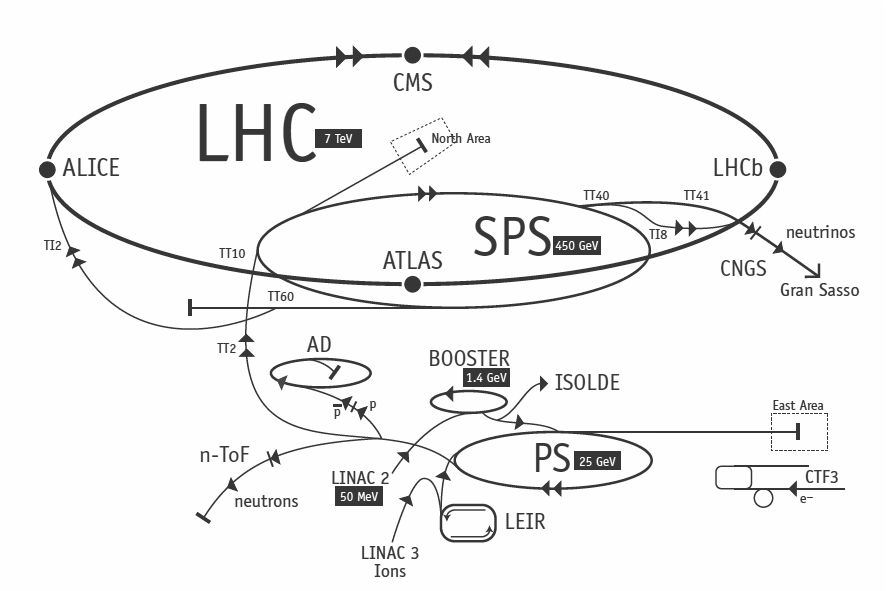
\includegraphics[width=1\textwidth]{Detector/figs/LHC_scheme.png}
\caption{Schematic of CERN accelerators~\cite{Christiane:1260465}.} 
\label{fig:lhc}
\end{figure}

Each beam consists of a series of proton bunches, up to a maximum of 2835. Each bunch consists of about $10^{11}$
protons and the bunch spacing is such that the nominal bunch crossing rate is 40 MHz. The beams are injected into
pre-accelerators and then pass into the LHC through the CERN acceleration system shown in Fig.~\ref{fig:lhc}. Protons are
produced from hydrogen gas and are initially accelerated to an energy of 50 MeV in a linear accelerator (LINAC).
Then they are injected into the Proton Synchrotron Booster (PSB), where they are boosted to an energy of 1.4 \gev,
into the Proton Synchrotron (PS) to 25~\gev~and into the Super Proton Synchrotron (SPS) to 450~\gev. Finally, protons
enter into the LHC storage ring, where they are accelerated from injection energy to the final one
by radio frequency (RF) cavities. The beams are steered around the ring by 8~T magnetic fields produced by 15~m long
superconducting niobium-titanium dipole magnets and focussed by quadrupole magnets. The LHC magnets
use a design in which both proton beam pipes are contained in the same housing, allowing a common liquid helium cooling
system to be used. The LHC began colliding proton beams in ``physics mode" in 2009 at a centre of mass
energy of $\sqrt{s} = 900$~\gev~and from April 2010 to November 2011 accelerated beams at $\sqrt{s} = 7$~\tev~(3.5~\tev~per
proton beam) with a maximum instantaneous luminosity of $3\cdot10^{33} \text{ cm}^{-2}\text{s}^{-1}$, while in
2012 the energy was increased to 8~\tev. The LHC maximum design energy is 14 TeV, and its design
luminosity is $10^{34} \text{ cm}^{-2}\text{s}^{-1}$. After a long shut down to upgrade and maintain the machine, a
new run started in June 2015, in which protons are collided at a centre of mass energy of $\sqrt{s} = 13$~\tev. At this
energy the total proton-proton cross-section is expected to be roughly 100 mb.
%, thus at the design luminosity the general purpose detectors will an event rate approximately $10^9$ inelastic events/s.

\section{The LHCb detector}

The LHCb detector~\cite{Alves:2008zz} was designed to study decays of $B$ and $D$ mesons,
mainly looking for CP-violating processes. In 2011, running at a centre of mass energy of 7 TeV, 
the cross-section for $b\bar{b}$ production was measured to be $284 \pm 53 ~\mu$b~\cite{Aaij:2010gn}, 
while it will be $\sim500 ~\mu$b at the current LHC energy, 13 TeV.
At these high energies, proton-proton interactions produce highly boosted virtual gluons which produce $b\bar{b}$
pairs at small angles, close to the beam pipe. For this reason the LHCb detector is designed to have a very forward angular
coverage. The detector is fully instrumented from 10 mrad to 300 mrad, corresponding to an interval
$2 < \eta < 5$, where $\eta$ is the ``pseudorapidity", a quantity defined as:
\begin{equation}
\label{pseudorap}
\eta = - \ln(\tan(\theta/2)),
\end{equation}
where $\theta$ is the angle between a particle's momentum and the beam direction\footnote{LHCb's coordinate 
system is right-handed, and has the $z$ axis in the direction of the beam, the $x$ axis directed to
the centre of the accelerator and $y$ is directed upward. Then we define $\theta$ as the angle with the beam
direction and $\phi$ as the position around the beam in the $xy$ plane, taking $\phi = 0$ on the $x$ axis.
The origin, $(x,y,z)=(0,0,0)$, corresponds to the centre of the interaction area.}.

\begin{figure}[h]
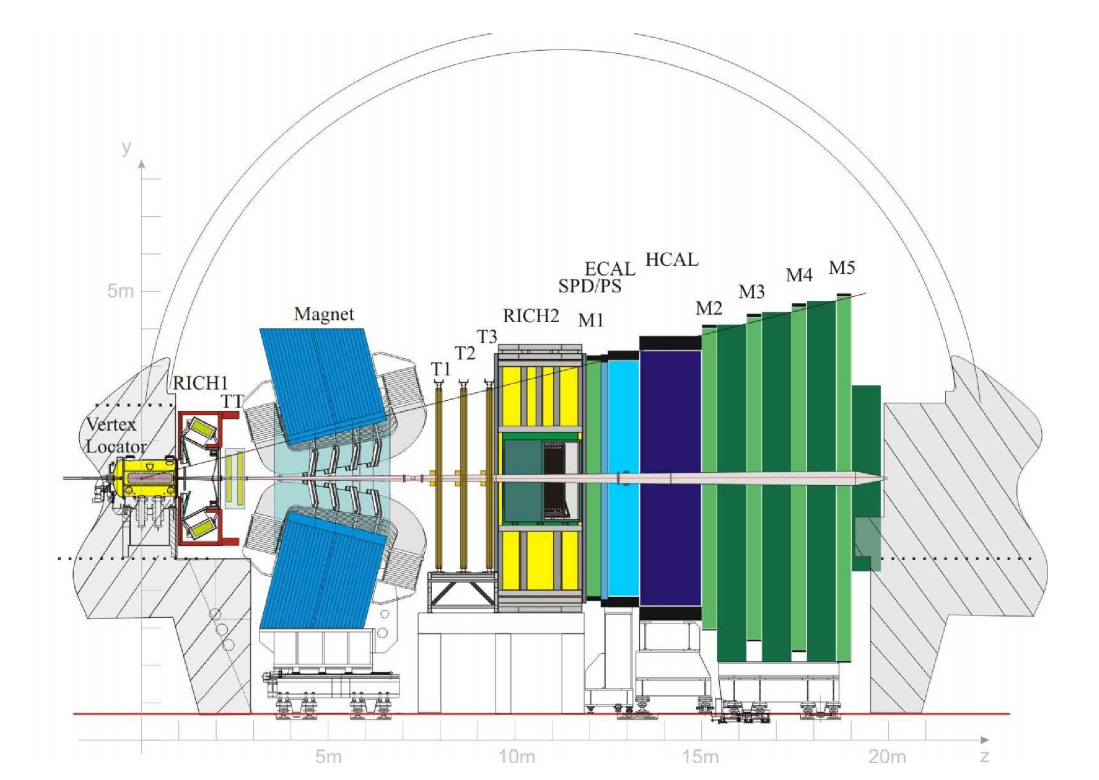
\includegraphics[width=1.\linewidth]{Detector/figs/LHCb_official.png}
\caption{A side view of the LHCb detector~\cite{Alves:2008zz}.}
\label{fig:lhcb}
\end{figure}

At LHCb's collision point the luminosity can be adjusted by displacing the beams from head on collisions
while keeping the same crossing angle. This allows the experiment to maintain an approximately constant instantaneous
luminosity, compensating for the reduction in beam intensity during extended operation periods. This also means that
the average number of interactions per bunch crossing can be regulated, which is important
because the detector efficiency, especially in detecting secondary vertices, decreases for events with an high number
of primary vertices (PV). Reducing the particle occupancy through the detector also keeps radiation damage to a minimum. 
Until the end of 2011 the instantaneous luminosity was $3 \cdot 10^{32}~\mbox{cm}^{-2}\mbox{s}^{-1}$, corresponding 
to an average number of 1.5 PVs per bunch crossing and at the end of 2011 LHCb had collected an integrated
luminosity of 1~\invfb. In 2012 the luminosity was increased and a further 2~\invfb of data were collected.

Experiments like BaBar at the Stanford Linear Accelerator (SLAC), Belle at KEK at J-PARC (Japan)
and the Tevatron experiments at Fermilab have made measurements in heavy flavour physics
which have so far been found to be consistent with the SM predictions. However, some of the deviations from the
SM are expected to be very small. Therefore LHCb was designed to make the most precise measurements
in heavy flavour physics to test the consistency of the SM and look for new physics.

The LHCb detector comprises a high-precision tracking system consisting of a silicon-strip
vertex detector surrounding the $pp$ collision point, and larger silicon-strip and drift tubes detectors located
on both sides of a dipole magnet with a bending power of about 4~Tm.
%The combined tracking system has momentum resolution $\Delta p/p$, that varies
%from 0.4\% at 5 $\mbox{GeV/c}^{2}$ to 0.6\% at 100 $\mbox{GeV/c}^{2}$. 
Charged hadrons are identified using information form two
Ring-Imaging Cherenkov detectors (RICH)~\cite{LHCb-DP-2012-003}. Photon, electron and hadron candidates are
identified by a calorimeter system and muons by a system composed of alternating layers of iron
and multi-wire proportional chambers~\cite{LHCb-DP-2012-002}. A schematic view of the detector is shown in Fig.~\ref{fig:lhcb}
and more details on each sub-detector are given in the following sections.

\section{The magnet}

Charged particle trajectories are deflected horizontally in the magnetic field
so that their momentum can be measured from the radius of curvature.
The LHCb dipole magnet is composed of two coils supported by an iron yoke
and is shaped to fit the LHCb angular acceptance. Unlike the other LHC experiments,
LHCb uses a warm magnet which can be easily ramped allowing the field polarity to be inverted periodically.
When the polarity is flipped, particles of a given sign are bent in the opposite direction.
This method is used to limit systematic uncertainties that arise due to performance
variations in different areas of the detector, which average out using data taken in both polarities.
A current of 5.85~kA flows in the magnet generating an integrated magnetic field of 4~Tm for 10~m long tracks.
In order to achieve the required momentum precision the magnetic field must be mapped with
a $10^{-4}$ precision. For this reason a grid of 60 sensors is positioned inside the magnet
and provides real time magnetic field maps.

\section{Tracking system}
\label{sec:tracking}

$B$ mesons have lifetimes of approximately 1.5 ps. At the LHC energies, this means that they travel about
1~cm before decaying to form a displaced vertex. To study specific decays, it is therefore important
to be able to separate the particles produced at the primary $pp$ vertex and at the $B$ decay secondary vertex (SV).
The tracking system consists of the Vertex Locator (VeLo), and four tracking stations:
the Tracker Turicensis (TT), which are located before the magnet and the T1, T2 and T3 stations,
located after the magnet. The latter three stations are in turn formed by two subsystems:
the Inner Tracker (IT) close to the beam-line, where the particle density is greatest, and
the Outer Tracker (OT) covering the rest of the acceptance.
%
\begin{center}
\begin{figure}[h!]
\centering 
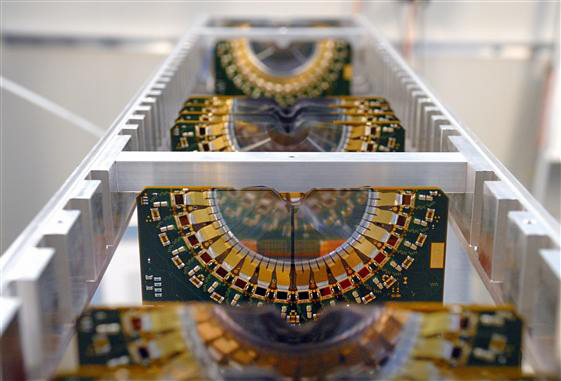
\includegraphics[width=0.49\textwidth]{Detector/figs/detector/VELO.png}
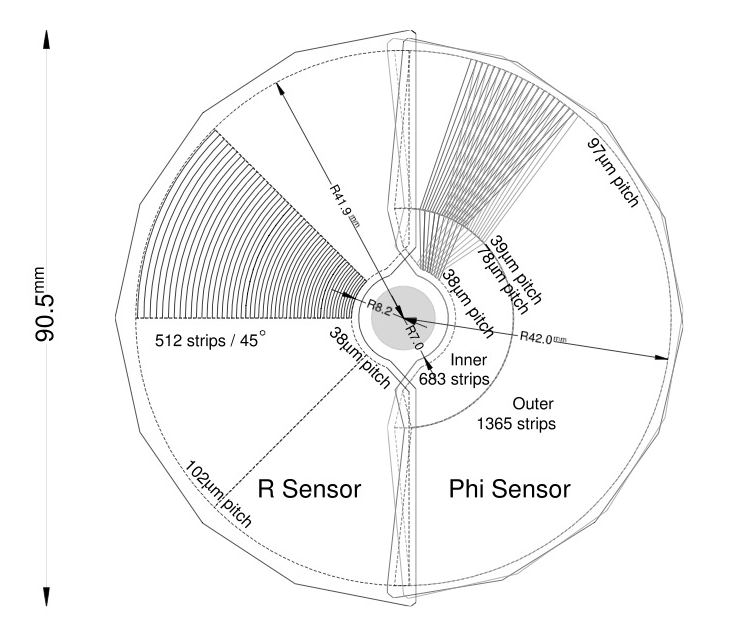
\includegraphics[width=0.49\textwidth]{Detector/figs/detector/VELO_scheme.png}
\caption{On the left VeLo sensors mounted in line and on the right a schematic view of one sensor~\cite{Alves:2008zz}.}
\label{VeLo}
\end{figure}
\end{center}
%
The VeLo accurately measures positions of tracks close to the interaction point which is essential to reconstruct
 production and decay vertices of bottom and charm hadrons. The VeLo is composed of 21
silicon modules that surround the beam axis and are positioned from $z = -18$~cm to $+80$~cm.
The sensitive region of the VeLo starts at an inner diameter of only 8~mm from the beam axis and it is able
to detect particles within a pseudorapidity range $1.6 < \eta < 4.9$. The VeLo is housed in its own
vacuum vessel of thin aluminium foil, which protects the vacuum of the beam pipe from any outgassing. 
The silicon layers composing the VeLo consist of two modules each including two types of sensors:
the $\phi$-sensor, which measures the azimuthal position around the beam, and the R-sensor, which measures
the radial distance from the beam axis. A sketch of the VeLo sensors is shown in Fig.~\ref{VeLo}. The sensors
are 300 $\mu$m thick and to ensure that they cover the full azimuthal angle the right-side module is placed
1.5~cm behind the left-side module on the $z$-axis and they overlap. There are two modules which cover the
backward direction and are used as a veto for multiple interactions; this is called the pileup system.
%
\begin{center}
\begin{figure}[h!]
\centering 
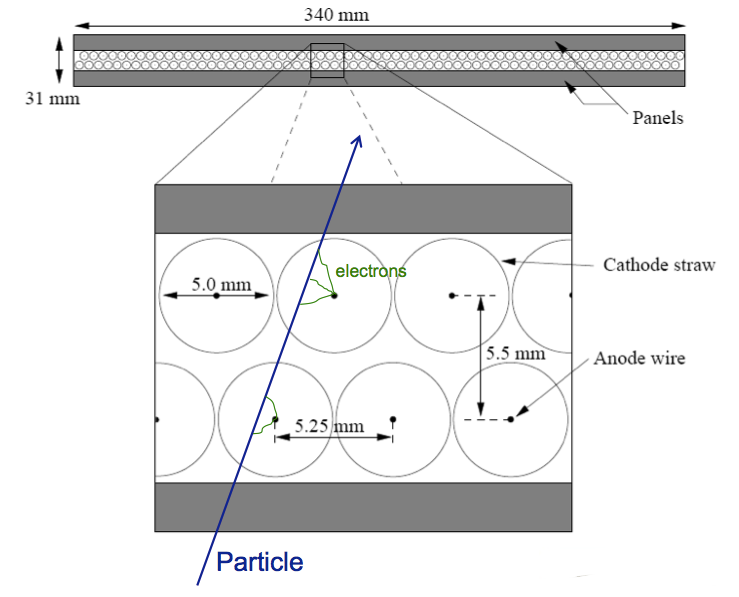
\includegraphics[width=0.8\textwidth]{Detector/figs/straw_tubes.png}
\caption{A sketch of the straw tubes which constitute the OT layers~\cite{Alves:2008zz}.}
\label{fig:straw:tubes}
\end{figure}
\end{center}
%
The IT and TT both use silicon strips and together constitute the silicon Tracker (ST). Straw tubes are instead used 
in the OT, of which a sketch is shown in Fig.~\ref{fig:straw:tubes}. The IT requires a higher inner granularity
because of the greater flux of particles close to the beam pipe. In fact, it covers only 1.3\% of the total
area of IT plus OT but it contains about 20\% of the tracks. Each ST station has four detection layers:
the first and last are vertical, measuring the track position in $x$, while the second 
and third layers are rotated by an angle of +5 and -5 degrees, which allows the measurement of the $y$ coordinate. 
The TT is placed upstream of the magnet to allow the reconstruction of tracks from low-momentum particles,
which are bent out of the downstream acceptance. Overall the tracking system provides a measurement of momentum, 
$p$,  with a relative uncertainty that varies from 0.4\% at 5~\gevc~to 1.0\% at 200~\gevc. 
The impact parameter (IP), namely the minimum distance of a track to a primary vertex, is measured 
with a resolution of $(15 + 29/\pt)$~$\mu$m, where \pt is the component of the momentum transverse to the 
beam, in \gevc. The $z$-axis position of a PV reconstructed with 35 -- 40 tracks can be measured with a precision 
of roughly 50 -- 60~$\mu$m. The decay products of $B$ mesons tend to have high IP values because the B decay imparts
transverse momentum to them. Therefore, accurate IP and vertex displacement measurements allow LHCb to distinguish 
effectively between $B$ meson decays and background processes. 
%In fact $B$ mesons typically travel $\sim 1$ cm in
%the detector before decaying into lighter particles, which .


\section{Calorimeters}
\label{sec:calorimeters}

In general the main purpose of a calorimeter system is to determine the energy of particles
but in LHCb it is mostly used to help the identification electrons and hadrons. 
Sampling calorimeters, as those used in LHCb, are composed of layers of absorber and active material.
Particles interact with the absorber layers and produce a cascade of secondaries that multiply quickly and are detected by the active part,
which is usually composed of scintillating layers. The light produced is detected by photo-multipliers (PMTs) and it is approximately
proportional to the energy of the deposited particles. Calibration is then used to translate the signal into an energy measurement. 
The LHCb's calorimeter system consists of the Scintillator Pad Detector (SPD), the Pre-Shower Detector (PS)
as well as the Electromagnetic Calorimeter (ECAL) and the Hadronic Calorimeter (HCAL).
A sketch of the LHCb calorimeters is shown in Fig.~\ref{fig:pi0_e_pid_perf}. 
The SPD/PS cells are read out with PMTs located outside the LHCb acceptance, while the ECAL and HCAL
have individual PMTs located on the modules. All four detectors are segmented, which allows the energy
deposits to be associated to the tracks detected by the tracking system. The segmentation of the cells
varies according to the distance from the beam pipe due to the different track density.

The most difficult identification in LHCb is that of electrons. The rejection of a high background of charged pions
is achieved using a longitudinal segmentation of the electromagnetic calorimeter which is provided by
the PS detector added in front of the main electromagnetic calorimeter, ECAL. Electrons also have to be 
distinguished from high energy $\pi^0$s and photons. For this purpose the SPD calorimeter, detecting charged particles,
is located in front of the PS and ECAL detectors. Figure~\ref{fig:pi0_e_pid_perf} illustrates how the ratio between the
energy detected in the ECAL and a particle's momentum allows the separation of electrons and hadrons.

\begin{figure}[t!]
\centering
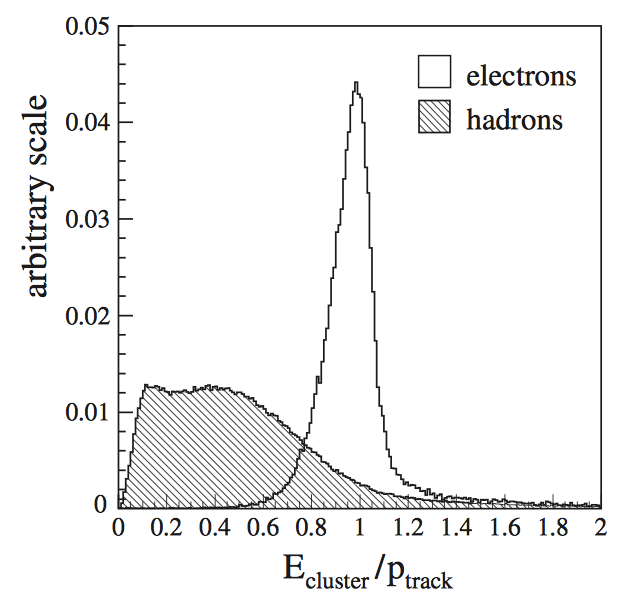
\includegraphics[width=0.4\textwidth,height=5.3cm]{Detector/figs/pi0_e_pid_perf.png}
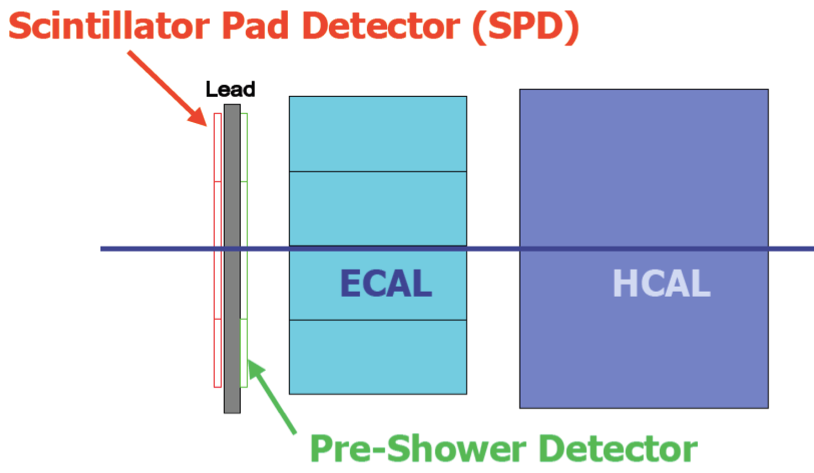
\includegraphics[width=0.59\textwidth]{Detector/figs/calo_layout.png}
\caption{(left) The ratio of the energy deposited in the ECAL and the particle momentum, which allows
the separation between electrons and hadrons~\cite{Alves:2008zz}. (right) A schematic of the LHCb's calorimeter system. }
\label{fig:pi0_e_pid_perf}
\end{figure}

The ECAL is formed by 66 lead layers (2 mm thick) separated by 4 mm thick plastic scintillator layers.
In order to obtain the highest energy resolution the showers from high energy photons 
must be fully absorbed. For this reason the ECAL has a thickness of 25 radiation lengths and its resolution is 
measured to be $\sigma_{\rm ECAL}(E) / E = 10\% / \sqrt{E(\gev )} \oplus 1\%$~\cite{Alves:2008zz},
which results in a mass resolution of $\sim 70$ \mevcc~for $B$ mesons and $\sim 8$ \mevcc~for \piz.
The HCAL is mainly used for triggering and it is similar to the ECAL but with 4 mm thick scintillator layers and 
16 mm thick absorber layers. The trigger requirements on the HCAL resolution do not depend on the containment of the hadron showers
as much as for the ECAL, therefore, due to space limits, its thickness is only 5.6 interaction lengths and its resolution is given by
 $\sigma_{\rm HCAL}(E) / E = 69\%/\sqrt{E(\gev )} \oplus 9\%$.

\subsection{Bremsstrahlung recovery for electrons}

Bremsstrahlung is an electromagnetic radiation produced by charged particles that undergo an acceleration. 
%because of the presence other charged particles. 
Typically electrons produce bremsstrahlung when deflected by atomic nuclei.
The probability of emitting bremsstrahlung radiation is proportional to the inverse of the squared mass of the
particle ($1/m^2$) and therefore it is most relevant for electrons.
%
\begin{figure}[h!]
\centering
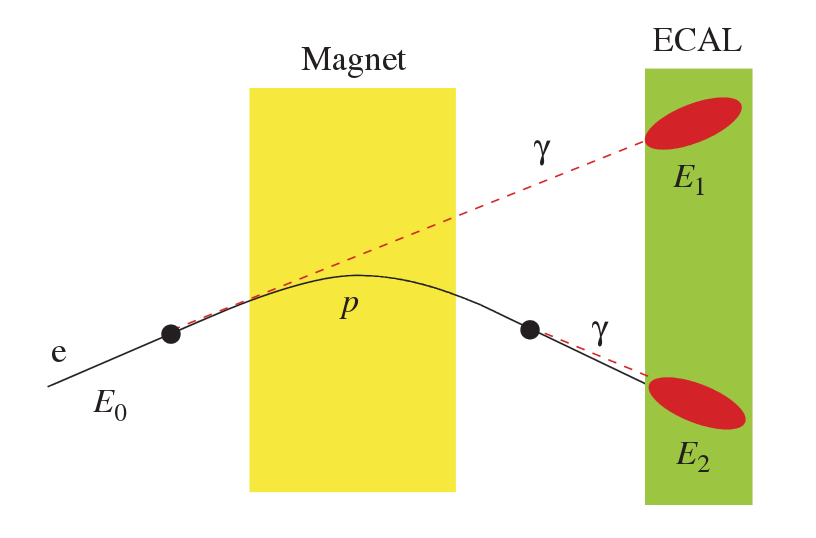
\includegraphics[width=0.55\textwidth]{RKst/figs/brem_recovery.png}
\caption{Schematic view of the bremsstrahlung recovery~\cite{Alves:2008zz}. }
\label{fig:bremreco}
\end{figure}
%
At LHC energies, if electrons radiate after the magnet, the photon will hit the same calorimeter cell
 as the electron and the energy will be automatically recovered, as illustrated in Fig.~\ref{fig:bremreco}.
However, if the photon is emitted before the magnet, the electron will be deflected by the magnetic
field whereas the photon will continue on its initial trajectory, with its energy being deposited in a different
part of the calorimeter. Missing this energy results in a poorer reconstructed invariant mass resolution, so it is
desirable to recover these bremsstrahlung photons. A tool for bremsstrahlung recovery is available
in the LHCb analysis software. This tool looks for other clusters in the calorimeter and, reconstructing the trajectory
of the electron, checks if they may be associated with emitted photons. The photon energy is then added to 
the electron and its momentum is recalculated. 
%Figure~\ref{fig:bremreco} displays a schematic view of the process. 
For more information see Ref.~\cite{LHCb:2003ab}.

\section{RICH}

The two RICH detectors are a special feature of LHCb, as it is the only experiment at LHC using them. 
These detectors take advantage of the Cherenkov radiation produced by particles passing through a medium
with speed higher than the speed of light in the medium. The Cherenkov light, as shown in Fig.~\ref{Cherenkov}, 
is produced in cones with a specific opening angle depending on the velocity of the particle. The relation
between the angle and the particle velocity can be written as 
%
\begin{equation}
\cos\theta = \frac{1}{\beta n},
\end{equation}
%
where $\beta = v/c$ and $n$ is the refraction index of the medium.
%
\begin{figure}[h!]
\centering
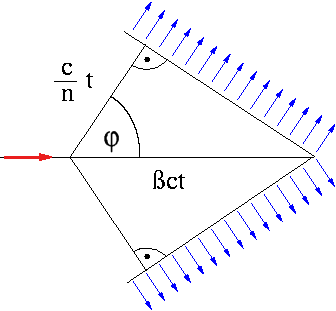
\includegraphics[width=0.45\textwidth,height=5.5cm]{Detector/figs/detector/Cherenkov.png}
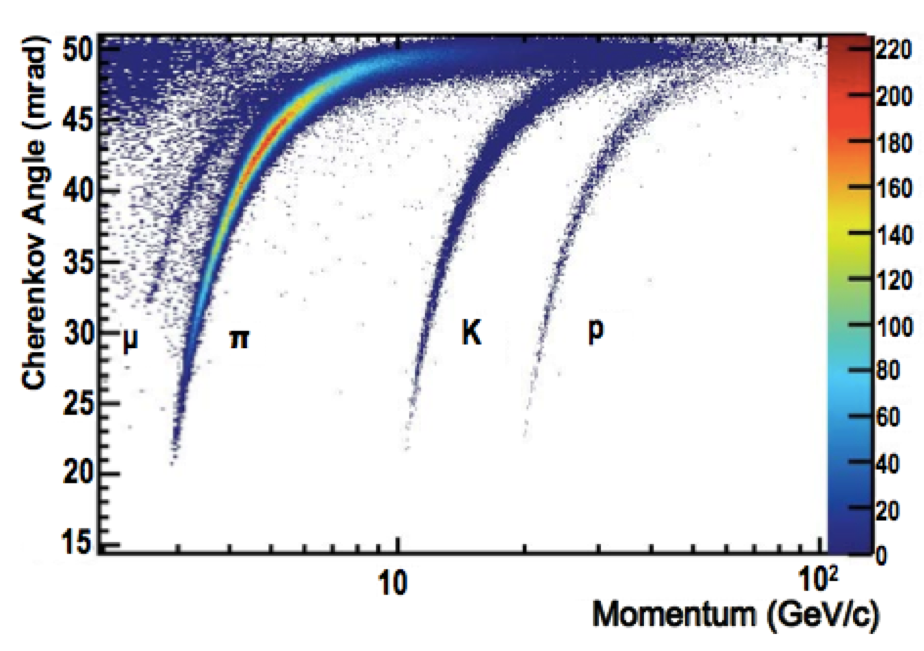
\includegraphics[width=0.45\textwidth,height=5.5cm]{Detector/figs/changle_vs_momentum.png}
\caption{(left) A sketch of Cherenkov light emission~\cite{Cherenkov_sheme}.
 (right) Measured Cherenkov angle as a function of particle momentum~\cite{Alves:2008zz}, where one
  can see that the study of the Cherenkov angle allows to distinguish particles' identities. }
\label{Cherenkov}
\end{figure}

RICH 1 is located before the magnet in order to cover a larger angular acceptance. Its purpose is to ensure
particle identification over the momentum range \mbox{$1 < p < 70$~\gevc}. It uses two radiators: $C_4F_{10}$ that covers
the momentum range $5-70$~\gevc~and silica aerogel which covers $1-10$~\gevc. RICH 2 is positioned after
the magnet and tracking stations and it identifies higher momentum particles from approximately 20~\gevc~up to beyond
100~\gevc~using $CF_4$ as a radiator.
The Cherenkov light produced when charged particles travel through the radiators, is reflected and focussed using
mirrors, which are tilted so that a ring image is reflected onto arrays of PMTs.
The radius of the ring can be used to measure the opening angle of the Cherenkov cone because of the known geometry.
The photo-detectors are located outside of the LHCb acceptance in order to reduce the amount of material that
the particles have to traverse. Pattern recognition algorithms are then used to reconstruct the Cherenkov rings.

%For particle identification a particle type hypothesis is assigned to each charged track found in the tracking stations.
%Initially the hypothesis is for a pion, which is the most common particle type. The corresponding expected number and
%Cherenkov radii of the resulting photons are calculated and the likelihood is calculated. The hypothesis is then changed
%and the likelihood is recalculated. The case with the largest increase in likelihood is kept.


\section{The muon system}

It is essential for many of the key physics analyses in LHCb to be able to identify muons in decay final states.
Muons are the most penetrating particles that can be detected at LHC experiments, so the muon chambers
are the farthest sub-detectors from the interaction point. The muon system consists of five stations (M1 - M5),
the first one being located before the calorimeters in order to improve \pt measurements. The remaining four stations
are behind the HCAL and are separated from each other by 80~cm thick iron blocks, which absorb
hadrons, electrons and photons to ensure that only muons reach the final muon station. 
A schematic of the muon system is shown in Fig.~\ref{fig:muonsystem}.
Only muons with a minimum momentum of 10~\gevc~traverse all of the
five stations and, for positive identification of a muon, the trigger requires a signal in each of them.
Each station has a detection efficiency of at least 95\% and the detectors also provide position measurements.
Since there is a larger particle flux close to the beam pipe, the stations are divided
into four concentric rectangular regions (R1-R4) with increasing cell size, which %according to the ratio 1 : 2 : 4 : 8.
results in a similar occupancy over the four regions. All of the muon stations use
Multi Wire Proportional Chambers (MWPC) except for the inner region of M1, where the particle flux is too high.
In this region triple-GEM (Gas Electron Multiplier) detectors are used because of their better ageing properties
as they have to withstand a rate up to $500 ~\mbox{kHz cm}^{-2}$ of charged particles. 
These detectors consist of three gas electron multiplier foils sandwiched between an anode and a cathode.
%In these detectors particles 
%traversing through the drift gap between the cathode and the first GEM foil produce ionisation electrons, which are then 
%attracted by electric fields though all of the GEM foils and multiply. They then drift into the anode inducing a signal on the 
%pads. A gas mixture of Argon, $CO_2$ and $CF_4$, is used to give a time resolution better than 3~ns.
%
\begin{figure}[h!]
\centering 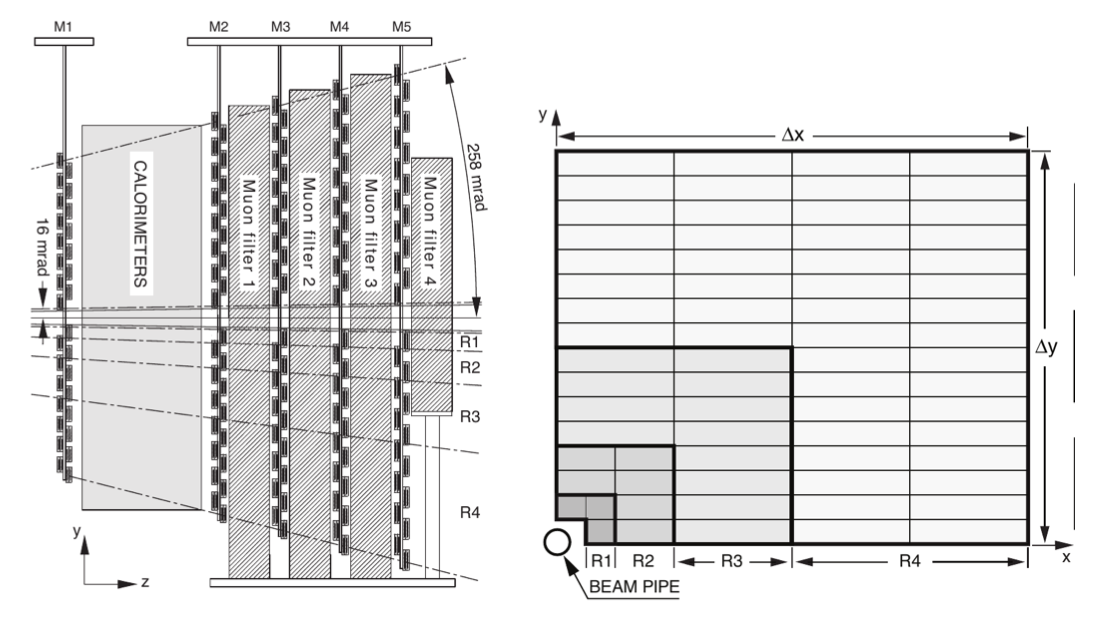
\includegraphics[width=1.0\textwidth]{Detector/figs/muon.png}
\caption{The LHCb muon system~\cite{Alves:2008zz}.}
\label{fig:muonsystem}
\end{figure}

\section{Particle identification}
\label{sec:PID_perf}

Particle identification (PID) is another important feature in LHCb and it is performed in various ways.
The electromagnetic calorimeters can distinguish between pions and electron, the muon chambers
identify muons and the RICH detectors can be used to identify 
more massive charged particles such as protons and kaons.

%The RICH assigns an ID to a track using a `global pattern recognition? algorithm [47].
The RICH assigns an identity (ID) to a track calculating the global likelihood for the observed distribution 
of hits being consistent with the expected distribution from various ID hypotheses.
The algorithm iterates through each track and recalculates the likelihood when the track PID hypothesis
is changed to that of an electron, muon, kaon or proton. For electrons and muons additional information
from the calorimeter and muon systems is also used. The hypothesis which maximises the likelihood
is assigned to the track.

%pion ID is used, as the pions are the most abundant particles.
To quantify the quality of the ID the pion hypothesis is used as a reference point and the probability
of a specific ID is given in terms of  Log-Likelihood difference between the given ID hypothesis and the pion one.
This variable is called Delta Log-Likelihood (DLL) and denoted with ``\verb!PID!".
For example,
\begin{equation}
\verb!PID!_K = \text{DLL}_{K-\pi} = \log(\mathcal{L}_K) - \log(\mathcal{L}_\pi)
\end{equation}
quantifies the probability of a particle being a kaon rather than a pion.
Figure~\ref{fig:pid_perf} shows the efficiency for correctly identifying and mis-identifying kaons and protons
as a function of the measured momentum of the particle. For kaons the efficiency drops at momenta below
10~\gev, where they fall below threshold for the gas radiators. 
The DLL cuts enable LHCb physics analyses to distinguish between kinematically similar decays 
with different final states. %, such as \Bz and \Bs mesons decaying into two hadrons.
For example, Fig~\ref{fig:pid_peaks} illustrates the power of particle identification,  showing how the application
of DLL cuts can be used to isolate $\Bz\to \pi^+\pi^-$ decays from other 2-body $B$ decays.
%
\begin{figure}[h!]
\centering
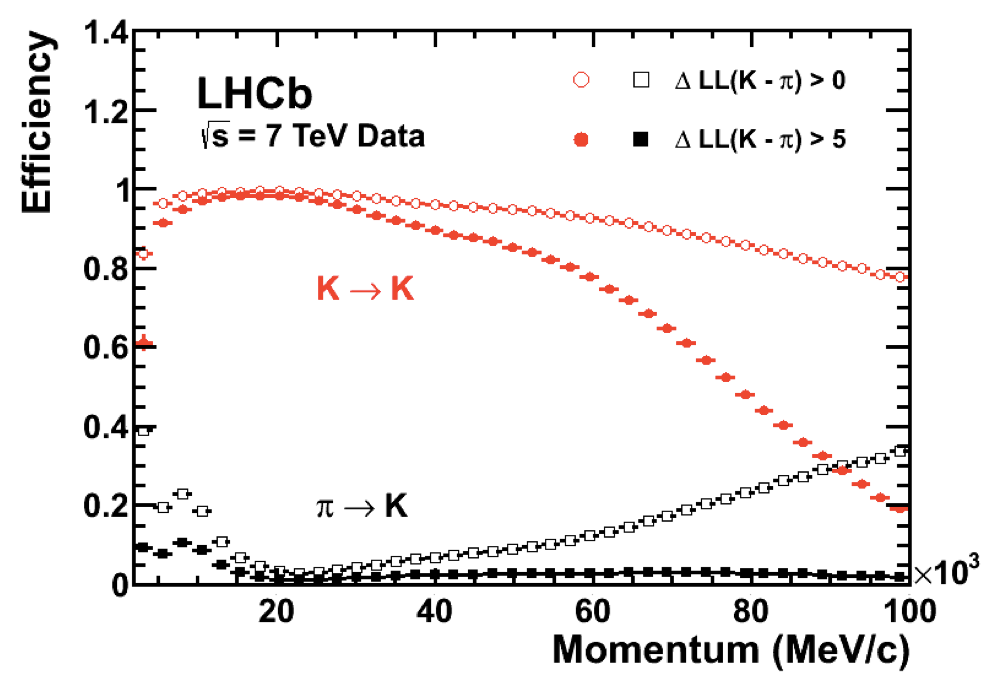
\includegraphics[width=0.49\textwidth]{Detector/figs/kaon_pid_perf.png}
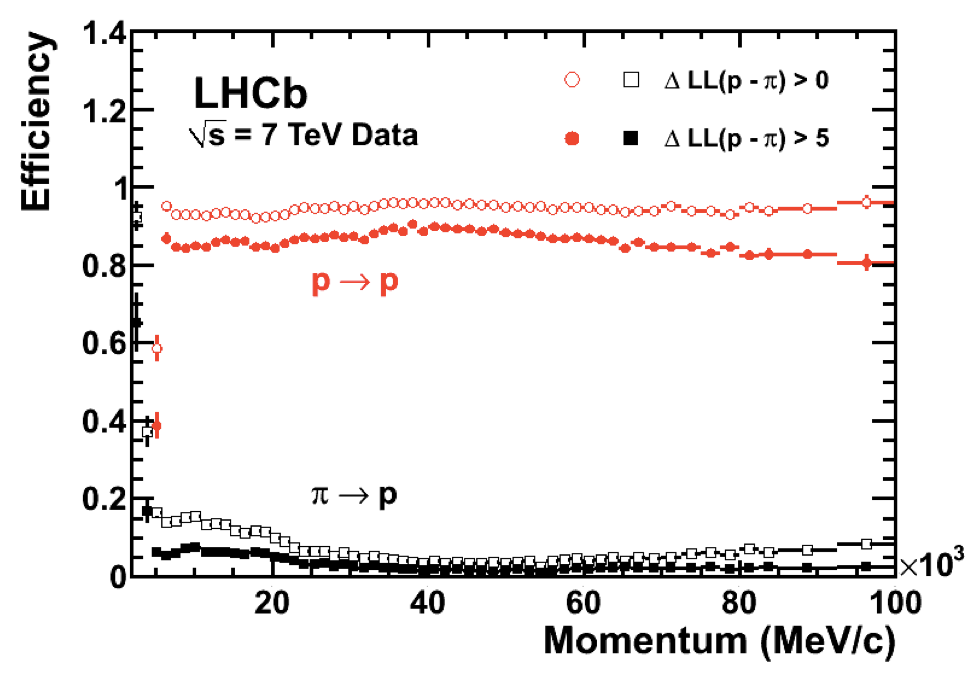
\includegraphics[width=0.49\textwidth]{Detector/figs/proton_pid_perf.png}
\caption{Particle identification performances for kaons (left) and protons (right) as a function
of the measured momentum of the particles~\cite{Alves:2008zz}. }
\label{fig:pid_perf}
\end{figure}
\begin{figure}[h!]
\centering
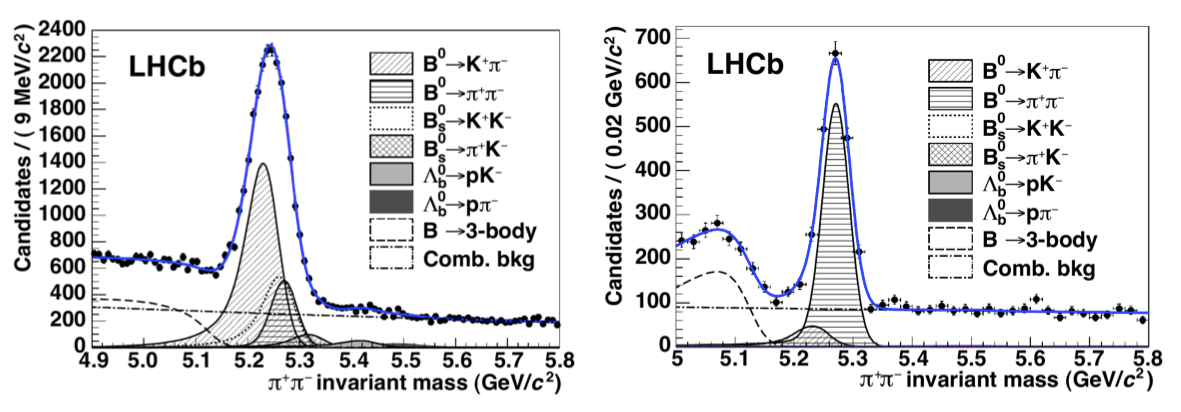
\includegraphics[width=1.\textwidth,height=5.5cm]{Detector/figs/pid_peaks.png}
\caption{Invariant mass peak of the $\Bz\to\pi^+\pi^-$ decay before (left) and
after (right) the application of PID requirements~\cite{Aaij:1978280}. }
\label{fig:pid_peaks}
\end{figure}

The identification of muons is particularly important in LHCb and it is quantified using two variables: the DLL$\mu$
and the \verb!isMuon! variable. The latter is a boolean variable determined by defining a `field of interest' around 
a track trajectory extrapolated through the muon chambers. The variable is set to true if hits in multiple muon stations are 
found in the field of interest.
%Tracks with higher momenta require hits in more muon stations.
%muDLL is the difference in the logarithm of the likelihood that the pattern of hits in the muon system is consistent with the extrapolated track being either a muon or a non-muon particle. The larger the value for muDLL the more ?muon-like? the track is.

\subsection{PID calibration}
\label{sec:PID_calib}

In order to be able to calculate detection efficiencies, a ``data-driven" method is used.
The calibration software is referred to as \verb!PIDCalib! package~\cite{Aaij:1978280}. 
This tool uses decays where final  particles can be identified thanks to their kinematic properties.
For example the $\KS\to\pi^+\pi^-$ decay has a clear signature with a displaced vertex
and can be easily singled out from other decays and used to test pion ID efficiency.
The narrow peaks of the $\jpsi\to\mumu$ and $\jpsi\to\ee$ decays allow
muon and electron efficiencies to be calibrated. A ``tag-and-probe" method is used in this case, 
where only one of the two leptonic tracks is reconstructed requiring the correct identity and the other
one is used to probe the PID efficiency. Finally,  $\phi\to KK$ samples and 
$D^{*+}\to D(\to K^-\pi^+)\pi^+$ decays, where the $D^{*+}$ is used to tag the decay,
are used to test the kaon efficiency. In all cases the residual background is subtracted using
the $_s\mathcal{P}$lot technique~\cite{sPlot}.


\section{Trigger and software}
\label{sec:det_trigger}

The LHCb trigger system~\cite{LHCb-DP-2012-004} consists of a hardware stage, L0, based on information
from the calorimeters and muon system, followed by a software stage, the High-Level Trigger (HLT), which applies 
a full reconstruction of the events. To increase performance, the HLT is further split into two stages, HLT1 and HLT2.
The HLT1 phase happens in real time and saves data to local disks while the HLT2 phase uses the resources
available during periods with no beam. The event selected by the HLT2 stage are then saved for offline analysis.
Figure~\ref{fig:triggerscheme} shows a schematic of the trigger system.
The bunch crossing frequency is 40~$\mbox{MHz}$, which corresponds to an instantaneous luminosity of 
$2 \cdot 10^{32} ~\mbox{cm}^{-2} \mbox{s}^{-1}$ for LHCb. About 15\% of the total number of
$\bquark\bquarkbar$ pairs produced will contain at least one $B$ meson with all of its decay products 
within the detector acceptance. This rate needs to be reduced to about 2~kHz at which the events
can be written to disk. 
%
\begin{figure}[h!]
\centering 
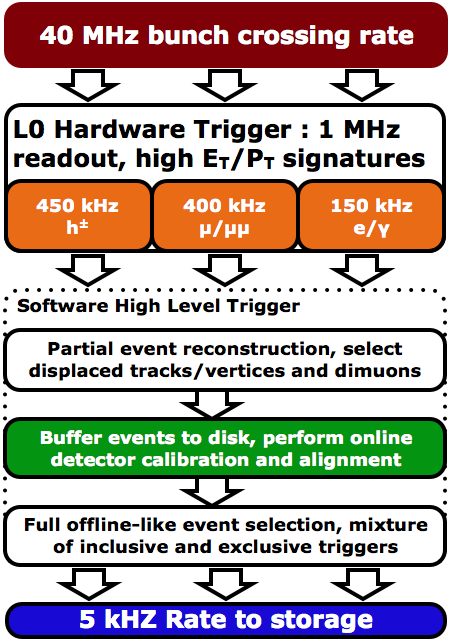
\includegraphics[width=0.5\linewidth]{Detector/figs/LHCb_Trigger_Split.png}
\caption{A schematic of the LHCb trigger system~\cite{Alves:2008zz}.}
\label{fig:triggerscheme}
\end{figure}

The L0 trigger reduces the rate of visible interactions from 10~MHz to 1~MHz.
Due to their high mass, $B$ mesons often produce particles with high energy and momentum.
Therefore the trigger selects events with large deposits in the calorimeter
or high \pt muons. The event is classified as \verb!L0Muon! if it was triggered due to information
from the muon detector, while the information from the calorimeters is used to divide the
events into five categories: \verb!L0Photon!, \verb!L0Electron!, \verb!L0LocalPion!, 
\verb!L0GlobalPion!, \verb!L0Hadron!. The PS detector information is converted to a photon flag 
(\verb|PS && !SPD|) or an electron flag (\verb|PS && SPD|). The ``local" label of the \verb!L0Pion! trigger 
refers to $\pi^0$ reconstructed though their $\gamma\gamma$ decay, where the two photons fall in the 
same ECAL element, they are labelled ``global" otherwise. The first four calorimeter triggers require 
energy clusters in the ECAL, while \verb!L0Hadron! requires clusters also in the HCAL. 
The HLT1 uses information from the VELO and trackers performing a partial reconstruction 
of the event and reduces the rate to 2~kHz by adding requirements on the IP and \chisq of tracks.
Finally, the HLT2 involves a full reconstruction of the event and includes many ``lines" designed 
to select specific decay structures.

LHCb has also developed an extended simulation software framework in order to reconstruct efficiencies and signal shapes.
In the simulation, $pp$ collisions are generated using $\textsc{Pythia}8$~\cite{Sjostrand:2006za,Sjostrand:2007gs} with a specific
LHCb configuration~\cite{LHCb-PROC-2010-056}. Decays of hadronic particles are described by $\textsc{EvtGen}$~\cite{Lange:2001uf},
and final state radiation is generated using $\textsc{Photos}$~\cite{Golonka:2005pn}. Finally, the interaction of the generated
particles with the detector and its response are implemented using the $\textsc{Geant4}$ toolkit~\cite{Allison:2006ve}
as described in Ref.~\cite{LHCb-PROC-2011-006}. For this analysis in this thesis, the ROOT framework~\cite{Brun:2000es} is
used to analyse data and the RooFit package to perform maximum likelihood fits. A multivariate analysis is also performed
based on the NeuroBayes package~\cite{Feindt:2006pm,feindt-2004}, which provides a framework for neural network training.

\section{Constrained kinematic fits}
\label{sec:DTF}

The resolution of key variables, such as the measured invariant mass of decaying particles,
can be improved by imposing constraints on the measured quantities to remove redundant degrees of freedom.
The four-momentum conservation can be ensured at each vertex and the origin and decay vertices of a particle 
are related via the momentum of the particle. Furthermore, additional constraints can be imposed due to a particular
decay hypothesis such as the known invariant masses of final and intermediate particles.
In order to do this the \verb!DecayTreeFitter! tool was developed by the BaBar experiment and later used by LHCb~\cite{Hulsbergen:2005pu}. 
The algorithm takes a complete decay chain and  parameterises it in terms of vertex positions, decay lengths and momentum parameters.
These parameters are then fit simultaneously, taking into account the relevant constraints, including the information
from photons. %To perform the fit efficiently a Kalman filter is used. 
Figure~\ref{fig:DTFeffect} illustrates the effect of
the application of the kinematical fit on the 4-body invariant mass of the final daughters of the $\Lb\to\jpsi\Lz$ decay.
The resolution in this case improves by over a factor of 2. Furthermore, the $\chisq$ from the kinematic fit
can be used to quantify the compatibility with a specific decay structure, which helps to separate candidates where random particles
from the event have been added to the decay tree, or where one or more particles is not reconstructed or mis-identified.
%
\begin{verbbox}DecayTreeFitter\end{verbbox}
\begin{figure}[h!]
\centering 
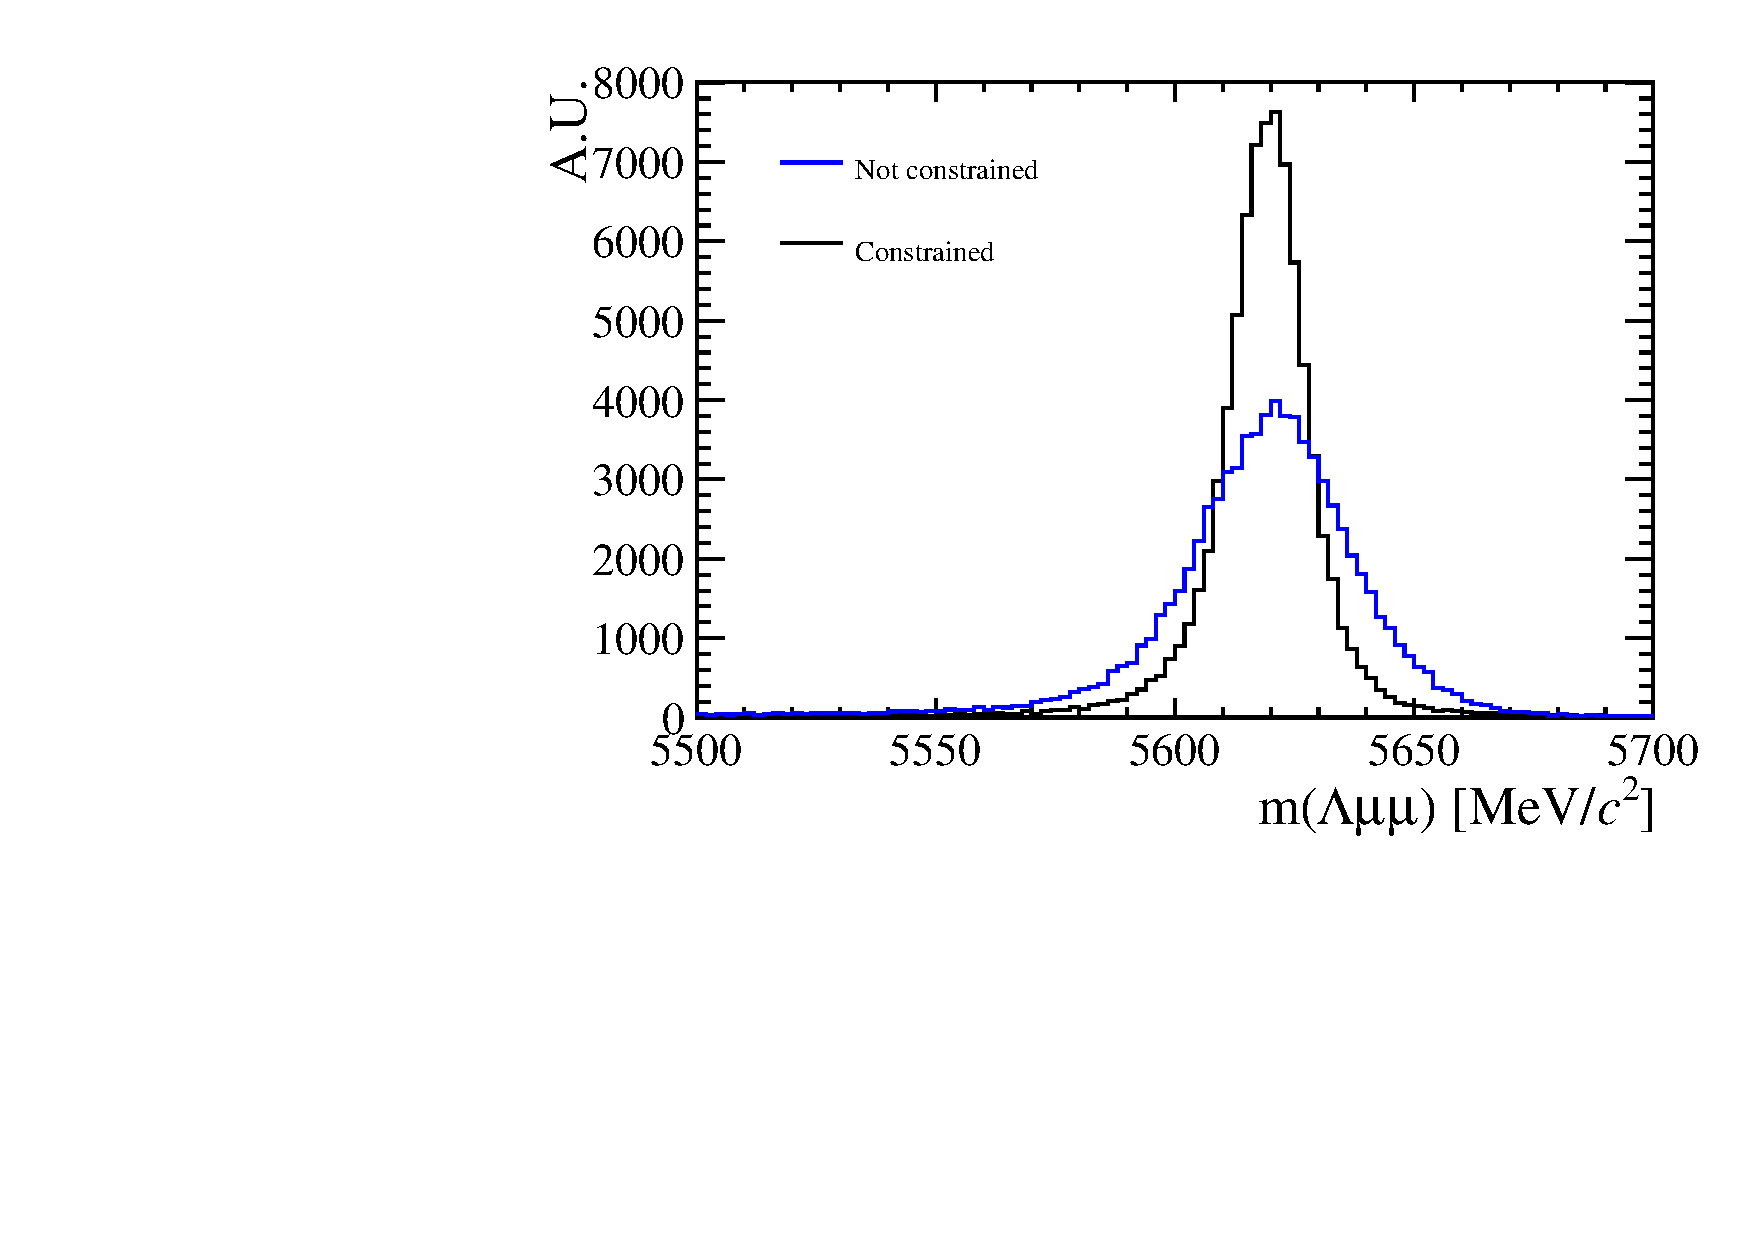
\includegraphics[width=0.7\textwidth]{Detector/figs/DTF_performance.pdf}
\caption{Invariant mass of the final daughters of simulated $\Lb\to\jpsi\Lz$ decays calculated
with and without constraints using the \theverbbox\! tool. }
\label{fig:DTFeffect}
\end{figure}

\section{Validation of hadronic processes in the simulation}
\label{sec:validation}

%As a service work for the experiment I have been working on the validation of the simulation of hadronic processes.
Particle-antiparticle asymmetries are of major interest for LHCb and detection efficiencies are usually obtained from simulation.
It is therefore important, in order to limit systematic uncertainties, to have a model that parameterises
correctly the cross-sections of particles and antiparticles or at least their ratio.

The LHCb simulation software propagates particles though the detector using the $\textsc{Geant4}$ toolkit~\cite{Alves:2008zz}.
This offers a variety of models for physics processes over a wide range of energies for both electromagnetic and strong interactions.
Given a combination of projectile, target and energy there can be several models applicable with different reliability
and computational costs. $\textsc{Geant4}$ provides a number of pre-packaged physics lists each representing
complete and consistent sets of models chosen to be appropriate for a given use case. In LHCb mainly two hadronic
physics lists are considered:
%
\begin{itemize}
\item {\bf LHEP} (Low and High Energy parameterisation): based on a parameterised modelling of all hadronic 
interactions for all particles. This list combines the High Energy parameterised model (HEP) and the low energy 
one (LEP). There is a sharp switch from the low to the high energy model at 25 GeV. The modelling of elastic 
scattering off a nucleus and of nuclear capture also proceeds via parameterised models.
%
\item { \bf FTFP$\_$BERT}: includes the following models:
%
\begin{itemize}
%
\item Bertini cascade model (BERT)~\cite{Bertini:1963zzc}, which simulates the intra-nuclear cascade, followed by pre-equilibrium 
and evaporation phases of the residual nucleus, for protons, neutrons, pions and kaons interaction with 
nuclei at kinetic energies below 9.9 GeV. The Bertini model produces more secondary neutrons and protons
than the LEP model, yielding a better agreement with experiment data.
%The Bertini-style cascade implements the inelastic scattering of hadrons by nuclei. Nucleons, pions, kaons and hyperons from 0 to 15 GeV may be used as projectiles in this model. Final state hadrons are produced by a classical cascade consisting of individual hadron-nucleon scatterings which use free-space partial cross-sections, corrected for various nuclear medium effects. The target nucleus is modeled as a set of 1, 3 or 6 spherical shells, in which scattered hadrons travel in straight lines until they are reflected from or transmitted through shell boundaries.
\item FTFP model, which implements high energy inelastic scattering of hadrons by nuclei using
the FRITIOF model~\cite{Andersson:1992iq}.
%
\end{itemize}
%It forms QCD strings by pairing a parton from the projectile hadron with a parton from a target nucleon. The strings are then excited by momentum exchange which can result in diffraction of the target or projectile or both. String masses are sampled and then the strings are decayed using the LUND fragmentation model. Tuning of the model parameters allow strings to be sampled down to quite low masses, which make the FTF model applicable down to 3 GeV. After the initial collision, the highly excited remnant nucleus is de-excited using the G4Precompound model. The FTFP model may be applied to incident nucleons, pions, kaons and hyperons from 3 GeV to several TeV.
%
The change between the two models happens with a linear shift from BERT to FTFP that starts at 4~GeV and ends at 5~GeV.
%
\end{itemize}

Figure~\ref{fig:models} summarises the composition of the different models.
%
\begin{center}
\begin{figure}[b]
\centering 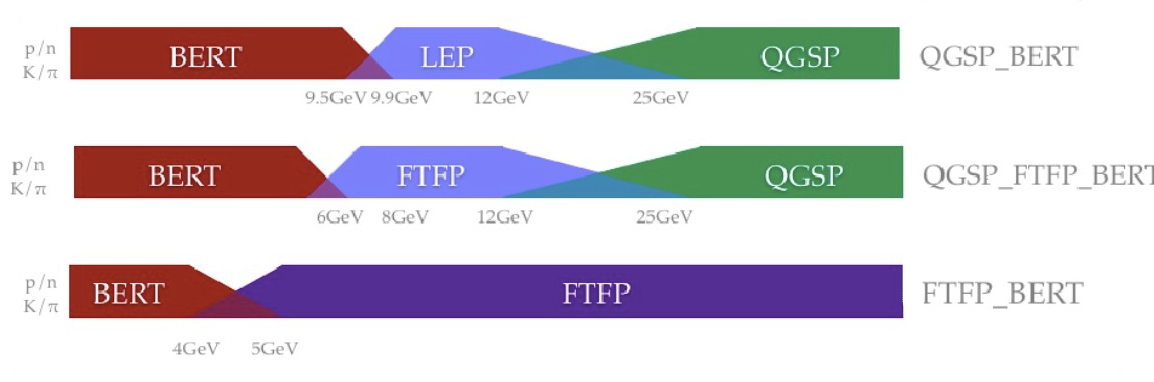
\includegraphics[width=0.9\textwidth,trim={0 1mm 0 0},clip]{detector/figs/validation/models.png}
\caption{Diagram of LHEP, FTFP$\_$BERT and QGSP$\_$BERT models' composition as a function of energy.}
\label{fig:models}
\end{figure}
\end{center}
%
When two models overlap in an energy interval the choice of the model
for each interaction is made using a random number: the probability to select each model varies linearly
from 0 to 100\% over the overlap range. Because of the differences of the two models in the overlap region,
unphysical discontinuities can be produced as a function of energy.

\subsection{Geometry and interaction probability}
\label{GeomandPint}

The results presented in the following sections are produced using the version v45r0 of the full LHCb framework
for simulation, \textsc{Gauss}~\cite{LHCb-PROC-2011-006}, which is interfaced to $\textsc{Geant4}$ v95r2p1.
A simple geometry setup is used in order to be able to calculate in a clean way the interaction cross-sections
in a specific material. This is consists of a series of rectangular boxes filled with the most relevant materials
for LHCb: aluminium, silicon and beryllium. For each material three boxes are defined with different thicknesses
(1mm, 10mm, 50mm). These values are chosen to be indicative of the amount of material present in the LHCb detector.

The simplest quantity available to extract the cross-section is the interaction probability, $P_{int}$, defined as:
%
\begin{equation}
P_{int} = \frac{N_{int}}{N_{tot}},
\end{equation}
%
where $N_{int}$ is the number of particles which interacted in the material and $N_{tot}$ is the number of generated particles.
%, usually set at 100k for this analysis.
As $\textsc{Geant4}$ provides an ID for the end process of a particle (\emph{e.g.} 121 for inelastic interaction, 111 for elastic, 
201 for decay) it is possible to distinguish the inelastic and elastic probabilities of interaction and therefore cross-sections.

To compare simulation and data the cross-section and $P_{int}$ are related through the following formula valid for thin layers:
%
\begin{equation}
\label{sigmaPint}
\sigma_{int} = \frac{A}{\rho N_A \Delta x} \cdot P_{int},
\end{equation}
%
where $\rho$ is the density of the material and A is its mass number, $\Delta x$ is the thickness of the considered layer and $N_A$ is the Avogadro number.

\subsection{PDG prediction}

In the Review of Particle Physics (PDG)~\cite{PDG2014} cross-sections of protons and neutrons are parameterised as:
%
\begin{align} 
\sigma_{tot}^{ab} = Z^{ab} + B^{ab}\log^2(s/s_M) + Y^{ab}_1(s_M/s)^{\eta_1} - Y^{ab}_2(s_M/s)^{\eta_2}, \\
\sigma^{\bar{a}b}_{tot} = Z^{ab} + B^{ab}\log^2(s/s_M) + Y^{ab}_1(s_M/s)^{\eta_1} + Y^{ab}_2(s_M/s)^{\eta_2},
\end{align}
%
where $s_M = (m_a + m_b + M)^2$ and $B^{ab} = \lambda \pi ( \frac{\hbar c }{M}  )^2$. Some of the constants in these 
equations are universal and valid for any kind of collision: M = 2.15, $\eta_1$ = 0.462, $\eta_2$ = 0.551, $\lambda$ = 1 
(for p, n and $\gamma$) and 1.63 (for $d$). The other ones are characteristic of each type of collision and are listed 
in Tab.~\ref{tab:PDGvalues}. In these formulae the particle-antiparticle asymmetry arises from the last term which has opposite
sign in the two equations. This term becomes less and less important with increasing energies. Therefore a net asymmetry 
is found at low energies, while the cross-sections tend to a common point at high energy and continue increasing logarithmically.
%
\begin{center}
\begin{table}[b]
\centering
\begin{tabular}{ $c | ^c | ^c | ^c }
\rowstyle{\bfseries}
Proj / Targ     &    $Z^{ab}$    &    $Y_1^{ab}$    &    $Y_2^{ab}$ \\
\hline
$\bar{p}$,$p$ / $p$     &    34.71   &     12.72     &    7.35 \\
$\pi^\pm$ / $p$           &     19.02  &      9.22    &   1.75  \\
$K^\pm$ / $p$             &     16.56  &      4.02      &    3.39 \\
$K^\pm$ / $n$              &     16.49 &    3.44        &    1.82 \\
$\bar{p}$,$p$ / $n$     &    35.00   &   12.19       & 6.62 \\
\end{tabular}
\caption{Values for the constants $Z^{ab}$, $Y^{ab}_1$ and $Y^{ab}_2$~\cite{PDG2014}, 
which parameterise hadronic cross-sections. }
\label{tab:PDGvalues}
\end{table}
\end{center}


\subsection{Validation results}

This section reports particle and antiparticle cross-sections and their ratios
compared, where available, with predictions and with data from the COMPASS experiment~\cite{Abbon:2007pq}.
%
Figure~\ref{fig:AllXsec} shows the probability of interaction for protons and anti-protons in 10~mm of aluminium
using the FTFP$\_$BERT and LHEP models compared with COMPASS data
%In this plot the colour of the marker indicates the material and the shape indicates the projectile. 
and Fig.~\ref{fig:ProtonsRatios} shows the ratios of $\sigma^{tot}_{\bar{p}} / \sigma^{tot}_{p}$
together with the PDG prediction. 
%
A difference of 40\% is found between the two considered models for 1~GeV incoming anti-protons.
This difference becomes negligible at higher energies. The discrepancies between the two physics lists
for kaons and pions are of a few percents (2--3\%) and usually constant with the energy. From the comparison 
with data and PDG predictions it can be qualitatively concluded that the FTFP$\_$BERT model gives a better
description of hadronic interactions at low energies, while both models give good results at high energy, above $\sim10$~\gev.

The tool developed for these studies is not limited to cross-sections but can also give information on other simulated quantities.
As an example, Fig.~\ref{fig:IDs_valdation} shows a comparison between the types of particles generated in inelastic
collisions of protons and anti-protons onto aluminium using different models. Physics lists can give very different results, 
for example the LHEP model does not produce photons in inelastic collisions. However, it is difficult to use these
quantities for validation as there are no data available for a comparison.


%\begin{table}[h!]
%\begin{center}
%\label{XsecRatios}
%\begin{tabular}{ | c | c | c | c | }
%\hline
%& $|p|$ (GeV) & LHEP & FTFP$\_$BERT \\ \hline
%\multirow{5}{*}{ \begin{sideways} ratio $\bar{p}$/$p$ \end{sideways}}
%& 1 GeV & $3.59 \pm 0.12$  & $1.82 \pm 0.06$  \\
%& 5 GeV & $1.41 \pm 0.05$  & $1.19 \pm 0.04$  \\
%& 10 GeV & $1.25 \pm 0.04$  & $1.15 \pm 0.04$  \\
%& 50 GeV & $1.11 \pm 0.04$  & $1.07 \pm 0.04$  \\
%& 100 GeV & $1.02 \pm 0.04$  & $1.07 \pm 0.04$  \\ \hline
%\multirow{5}{*}{ \begin{sideways} ratio $\pi^{-}$/$\pi^{+}$ \end{sideways}}
%& 1 GeV & $1.10 \pm 0.03$  & $0.98 \pm 0.03$  \\ 
%& 5 GeV & $1.07 \pm 0.03$  & $1.00 \pm 0.03$  \\ 
%& 10 GeV & $1.06 \pm 0.03$  & $0.95 \pm 0.03$  \\ 
%& 50 GeV & $1.06 \pm 0.03$  & $0.97 \pm 0.03$  \\ 
%& 100 GeV & $0.97 \pm 0.04$  & $1.02 \pm 0.03$  \\ \hline
%\multirow{5}{*}{ \begin{sideways} ratio $K^{-}$/$K^{+}$ \end{sideways}}
%& 1 GeV & $2.68 \pm 0.10$  & $1.61 \pm 0.05$  \\ 
%& 5 GeV & $1.37 \pm 0.05$  & $1.21 \pm 0.04$  \\ 
%& 10 GeV & $1.22 \pm 0.04$  & $1.16 \pm 0.04$  \\ 
%& 50 GeV & $1.13 \pm 0.04$  & $0.99 \pm 0.03$  \\ 
%& 100 GeV & $0.94 \pm 0.04$  & $1.05 \pm 0.04$  \\ \hline
%\end{tabular}
%\caption{Ratio of the total probability of interaction of antiparticle over particle for different energies and particles.}
%\end{center}
%\end{table}

\begin{center}
\begin{figure}[h]
%\centering 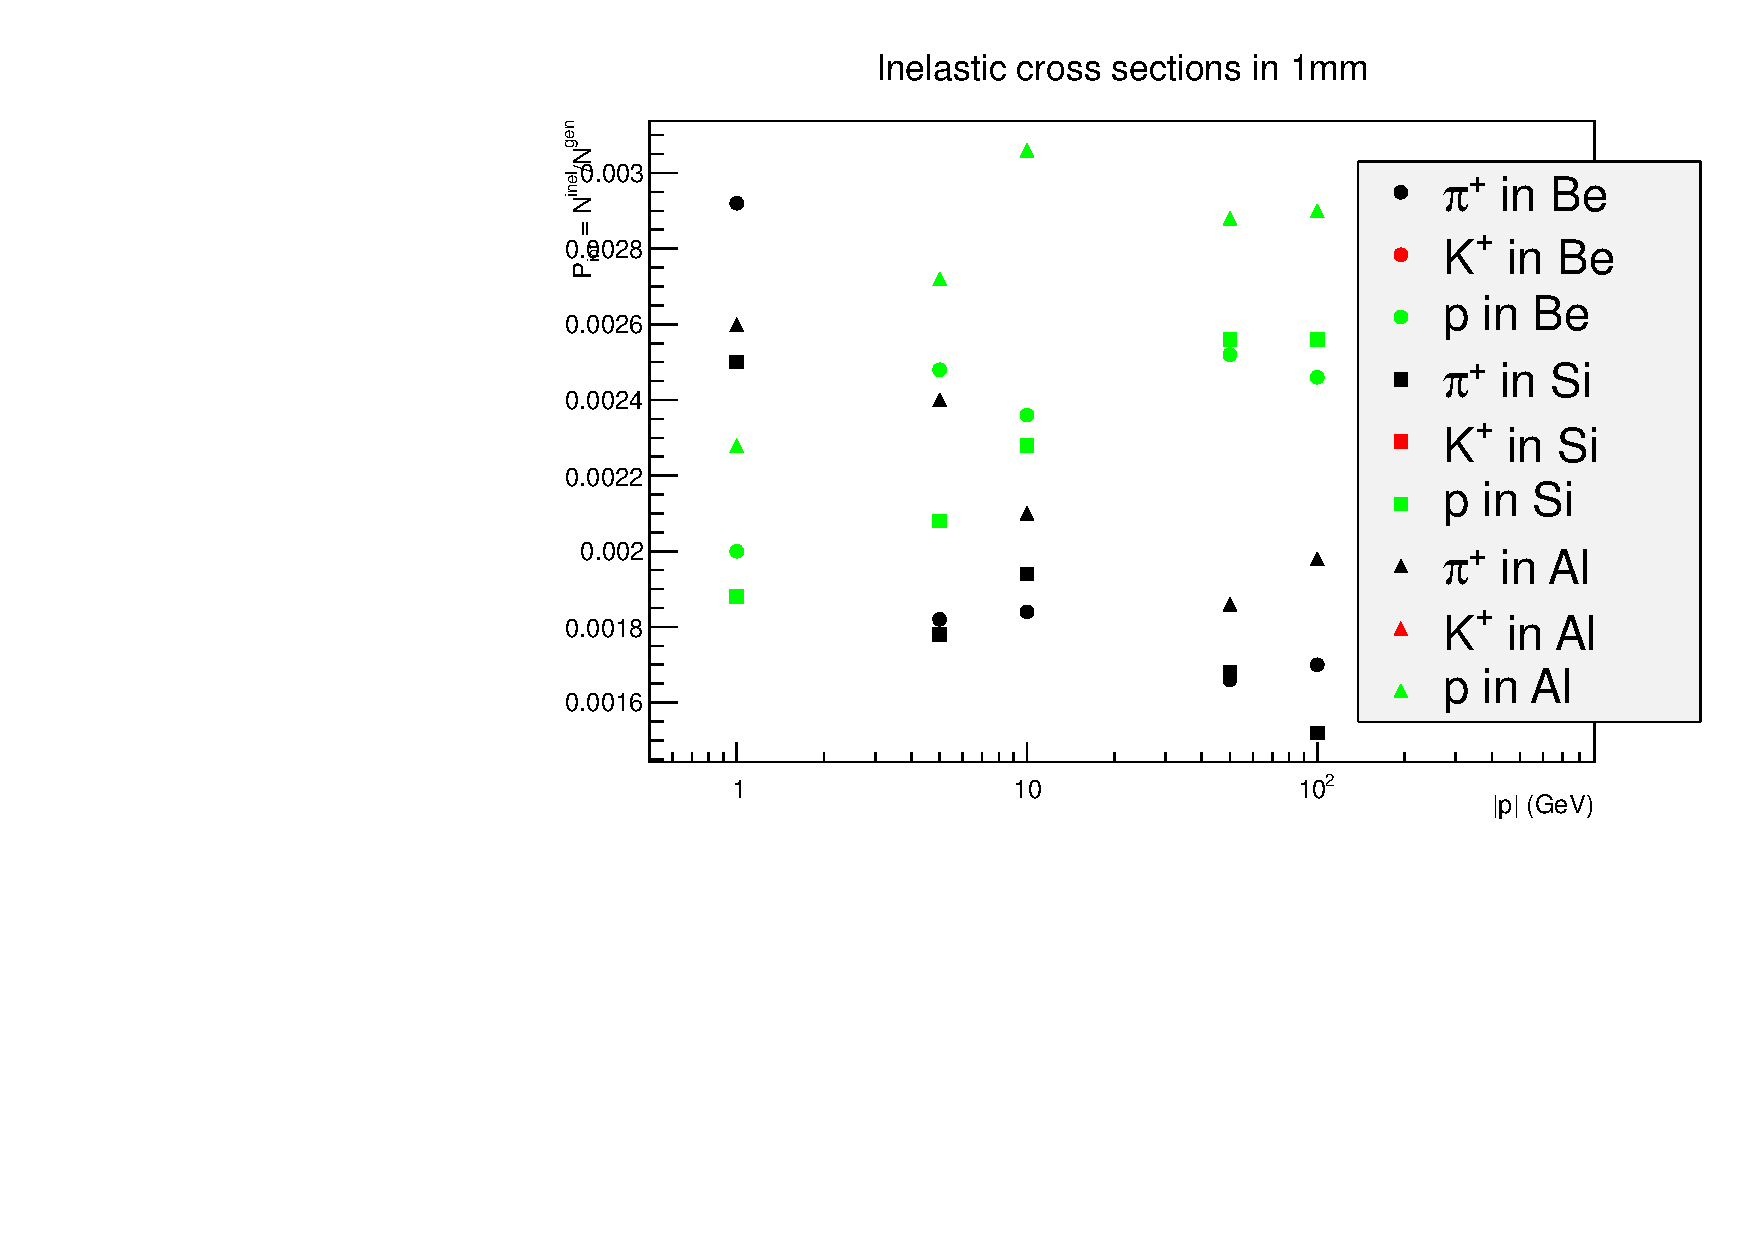
\includegraphics[width=0.8\textwidth]{Detector/figs/validation/Xsec_PosBERT1mm.pdf}
%\caption{cross-sections for $p$, $K^+$ and $\pi^+$  in 1mm of Al, Si and Be as a function of energy.}
\centering 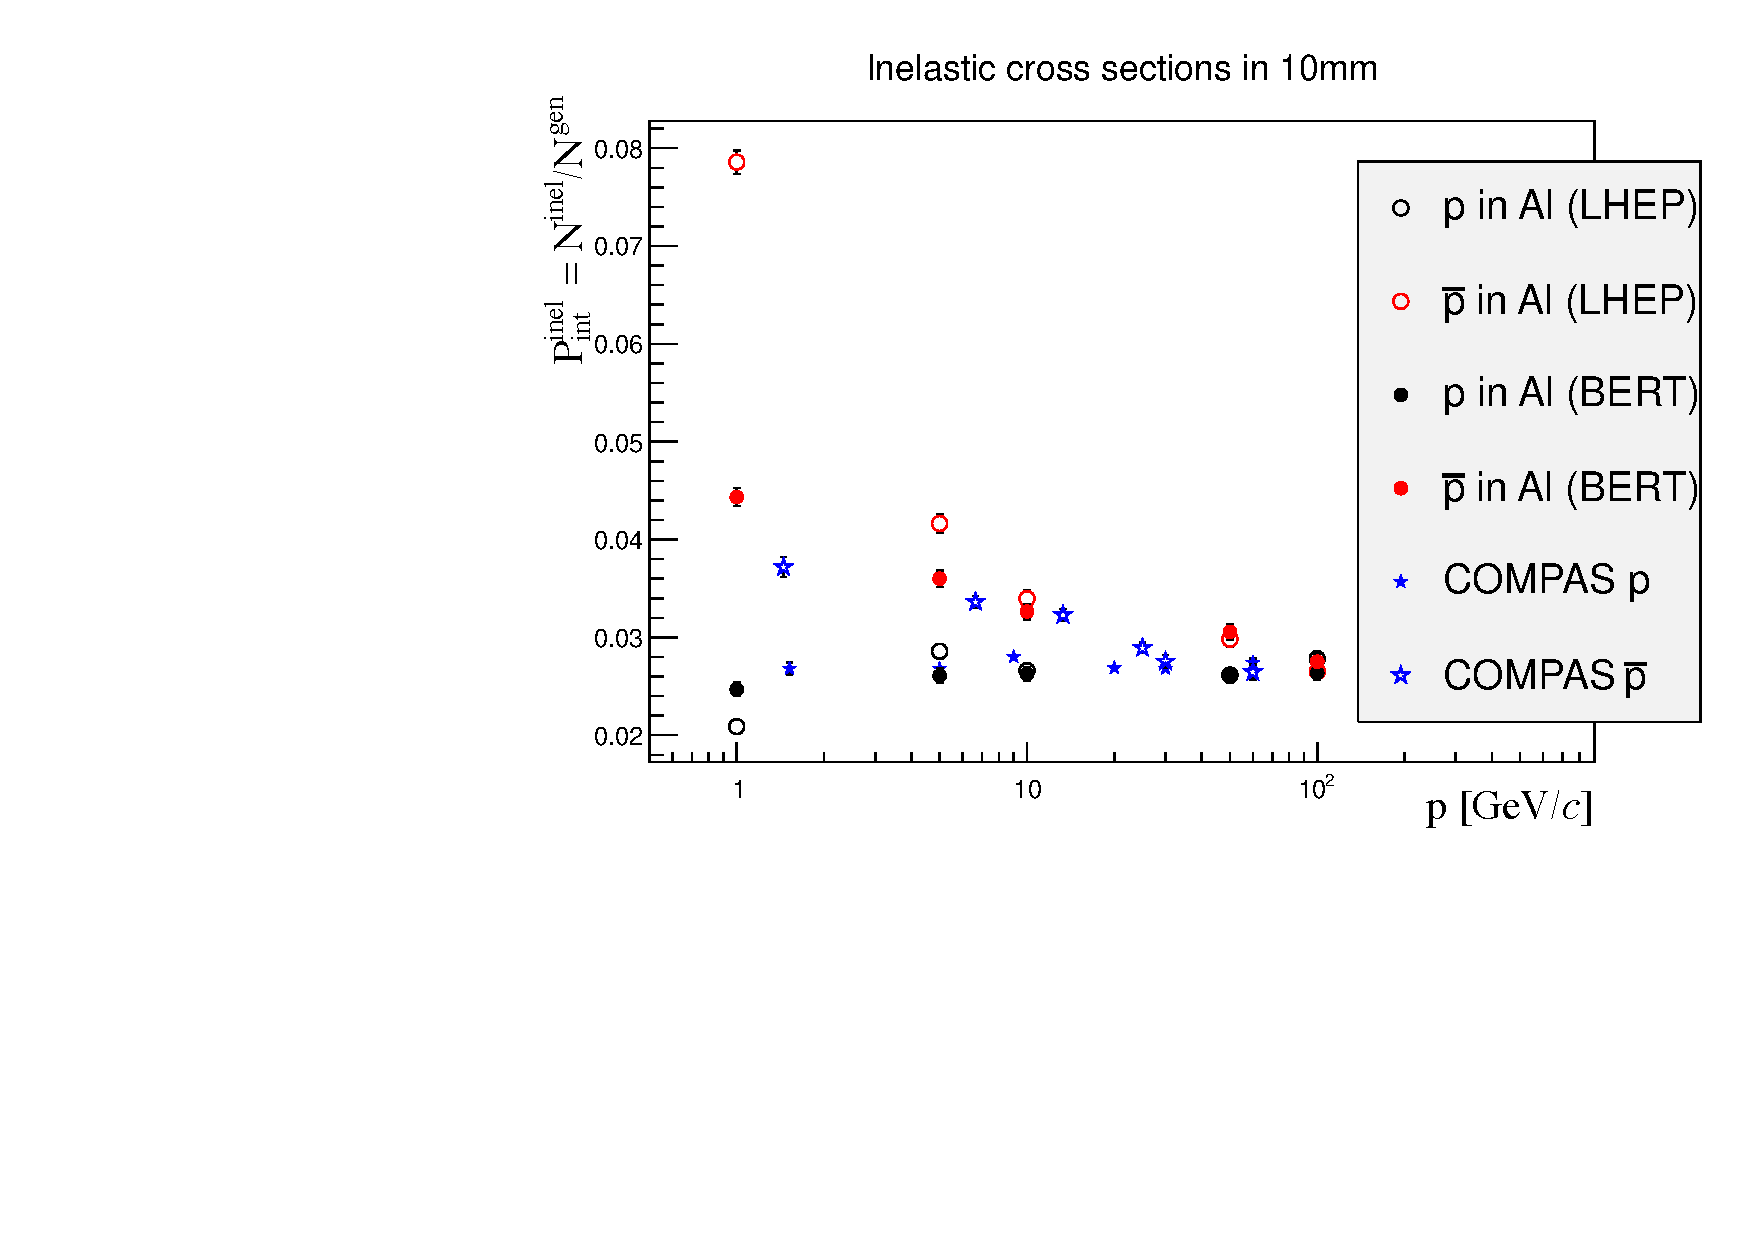
\includegraphics[width=0.8\textwidth]{Detector/figs/validation/General/pCompData_10mm.pdf}
\caption{Probability of interaction for protons and anti-protons in aluminium as a function of the projectile momentum.
Two physics lists are used to generate events that can be compared with data from the COMPASS experiment.}
\label{fig:AllXsec}
\end{figure}

\begin{figure}[h!]
\centering 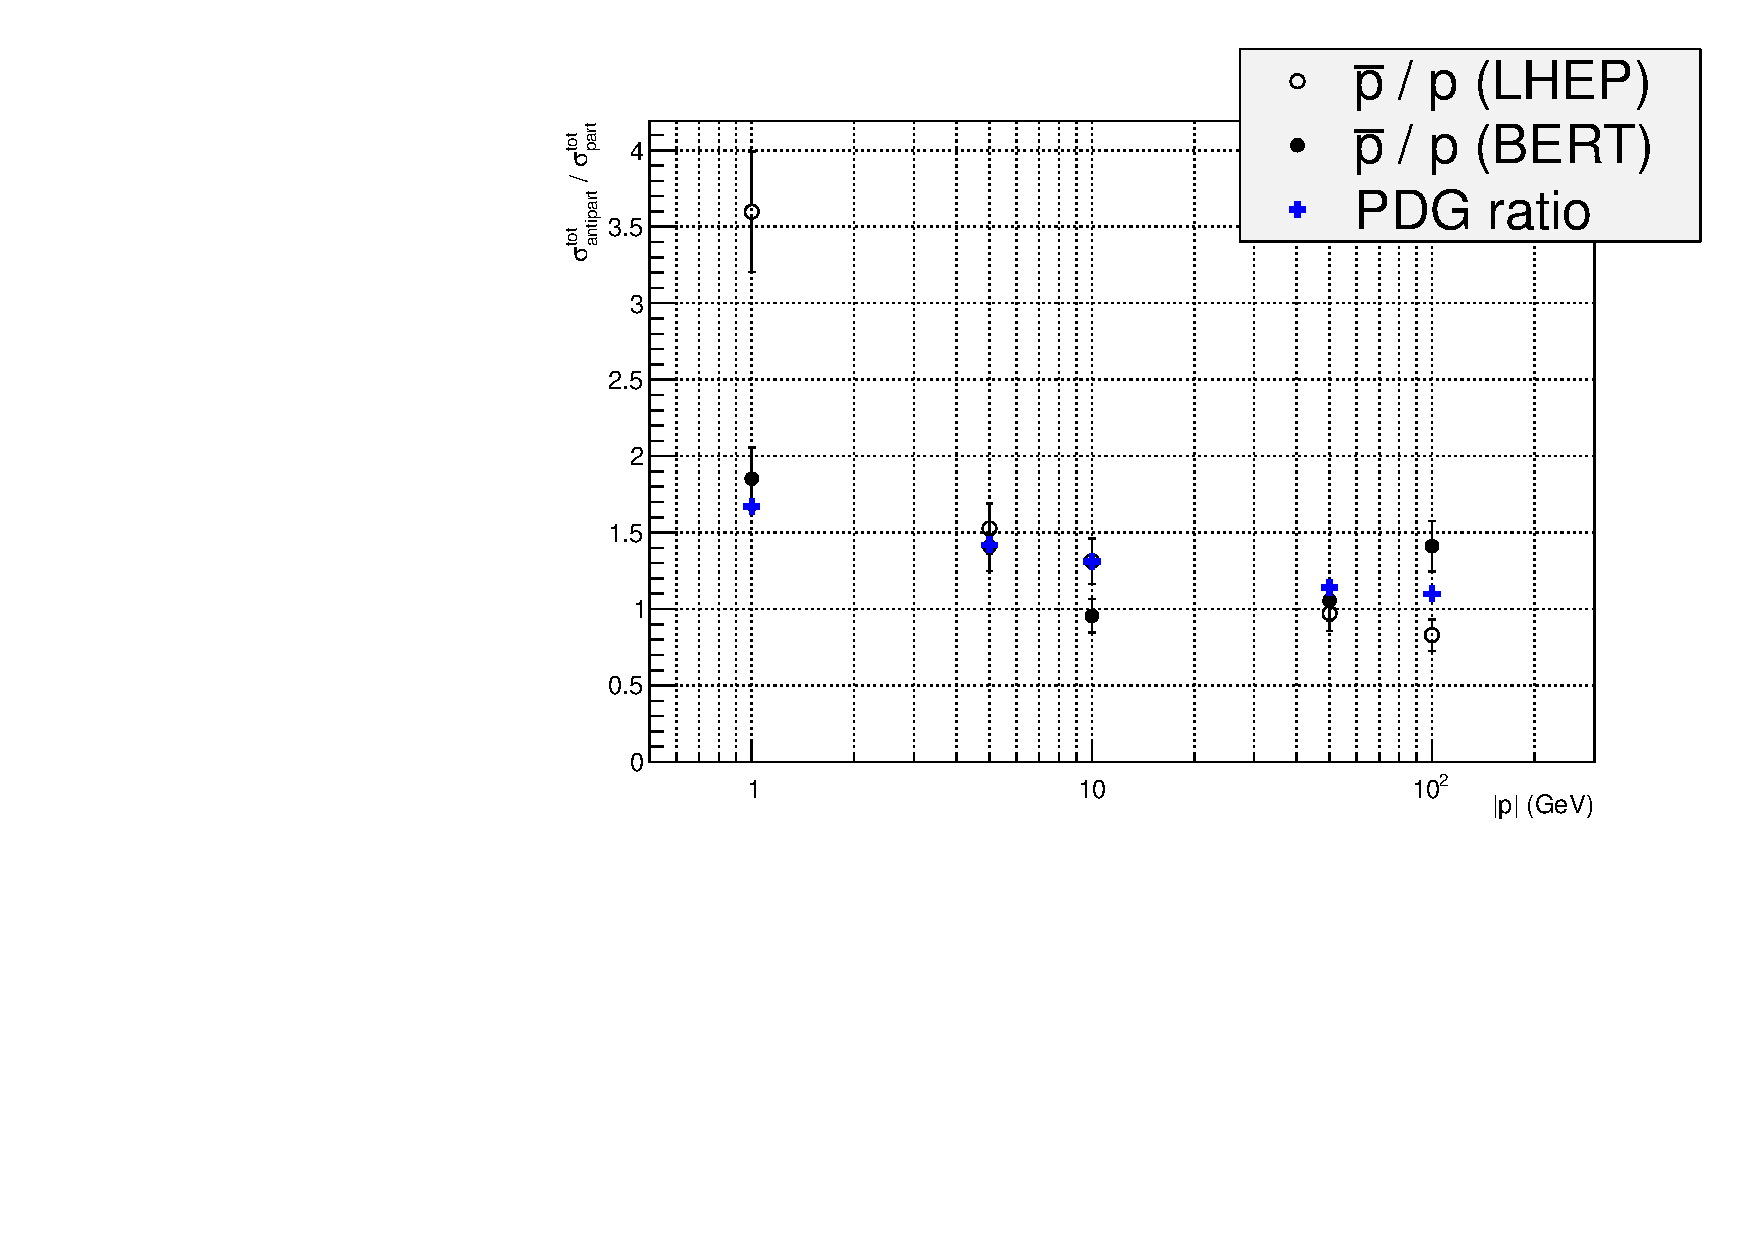
\includegraphics[width=0.8\textwidth]{Detector/figs/validation/ProtonsRatio_2.pdf}
\caption{Ratio of antiproton over proton total interaction cross-section as a function of energy compared with PDG predictions.}
\label{fig:ProtonsRatios}
\end{figure}

\begin{figure}[h!]
\centering 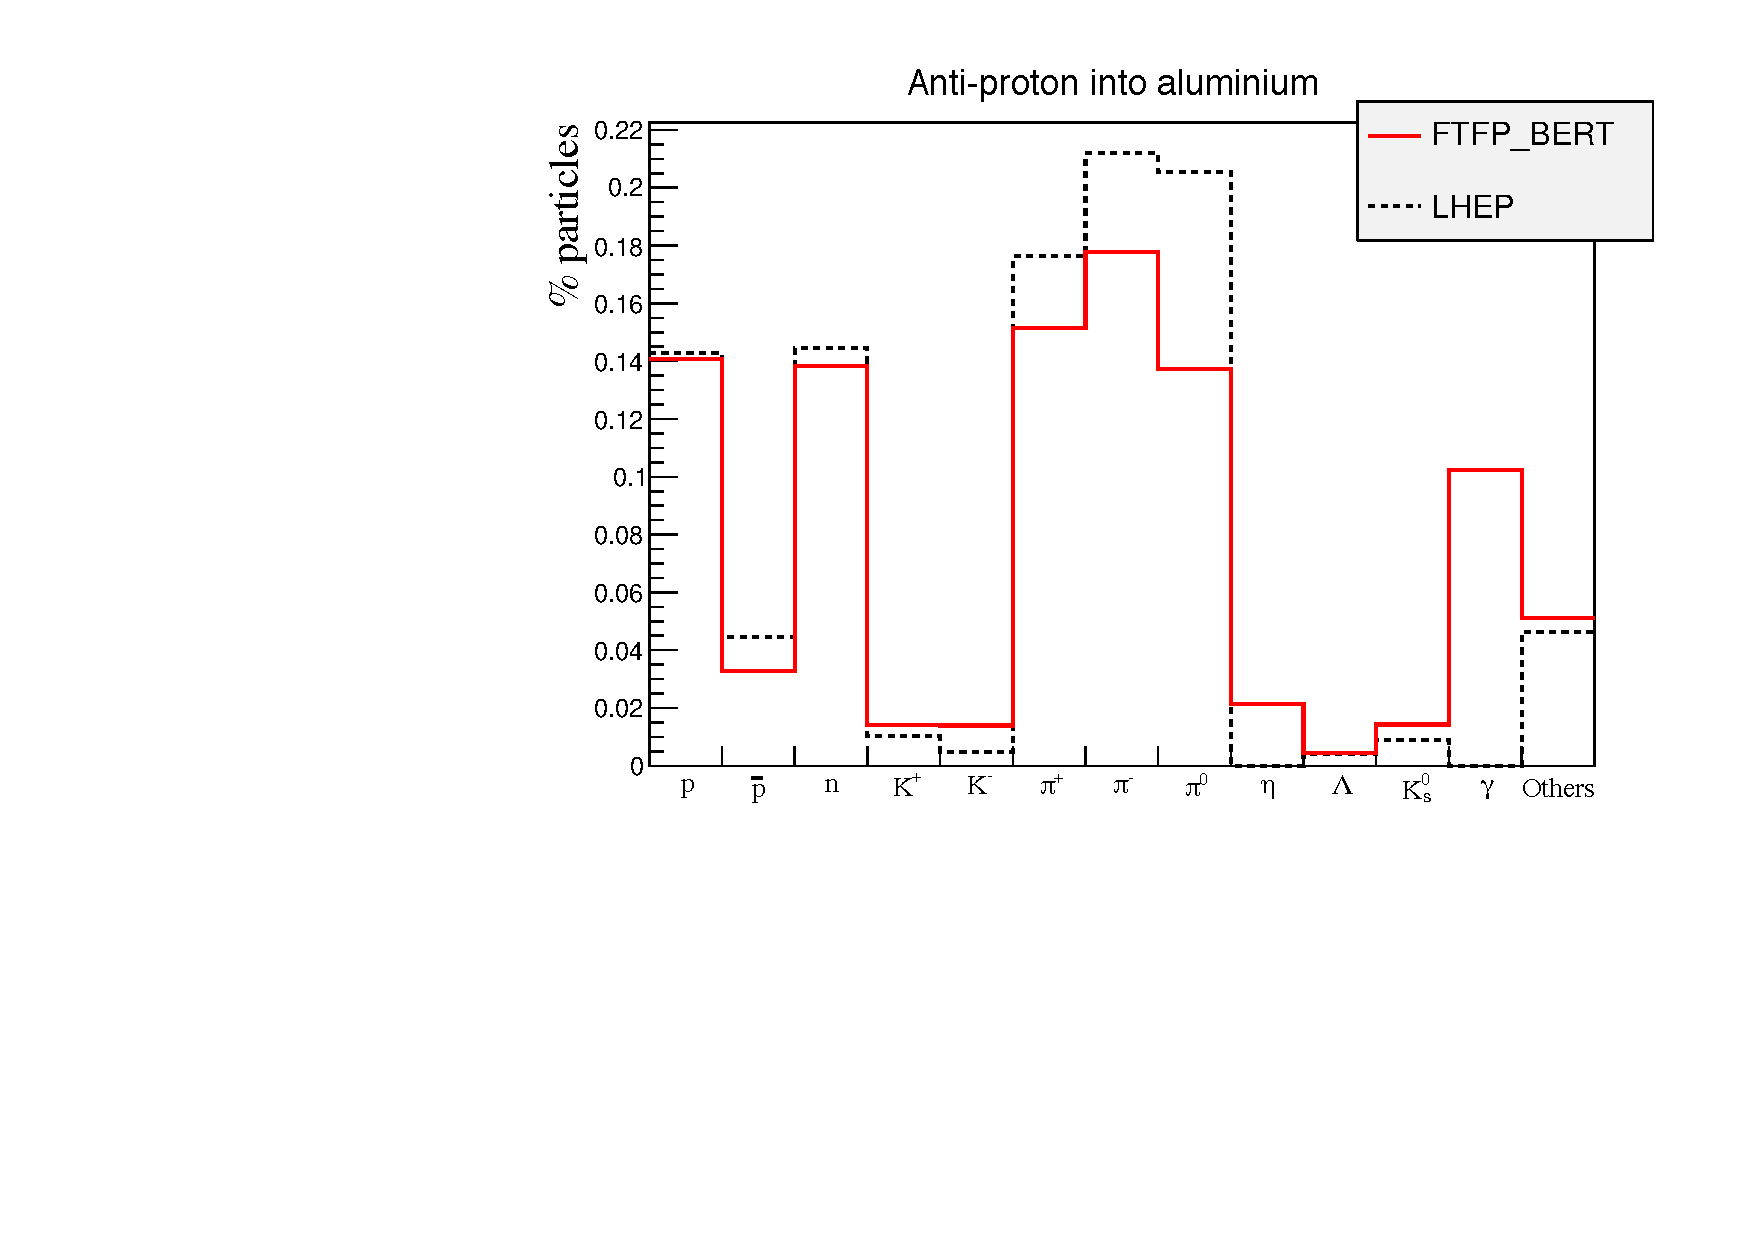
\includegraphics[width=0.9\textwidth]{Detector/figs/validation/perc_pbarcomp.pdf}
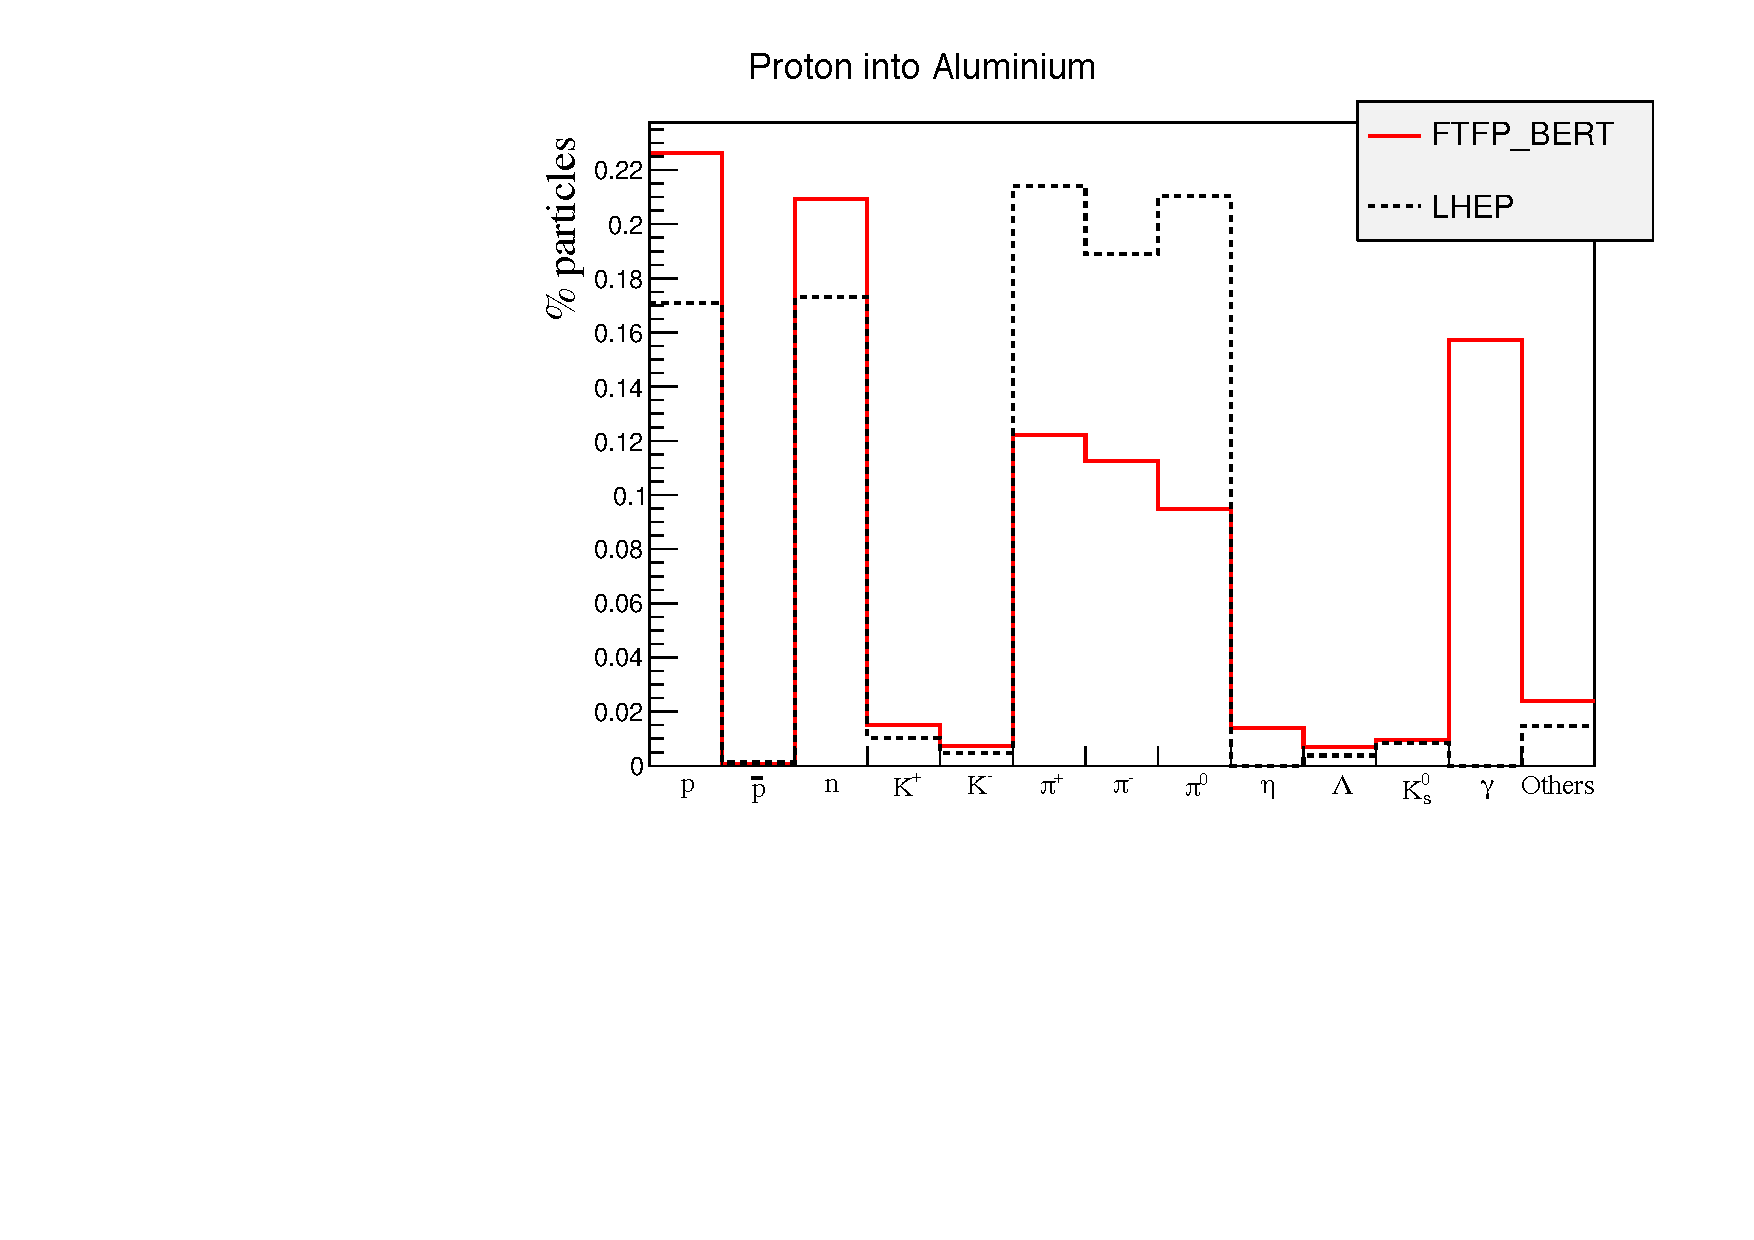
\includegraphics[width=0.9\textwidth]{Detector/figs/validation/perc_pcomp.pdf}
\caption{Composition of secondary particles produced in 100~\gev~ protons (top)
and anti-protons (bottom) collisions in 1~mm of aluminium.}
\label{fig:IDs_valdation}
\end{figure}
\end{center}

\clearpage
\section{Material budget studies}

It is important for many analysis to quantify the amount of material present in the detector, for example to estimate
the amount of multiple scattering. In \textsc{Geant4} particles are propagated in steps
through the detector and for each step the framework analyses the geometry to understand in what material
the particle is and modifies its trajectory accordingly. A tool was developed where neutrinos are
used as probes to scan the detector summing the radiation length seen at each step up to a certain point.
%
\begin{figure}[b]
\centering 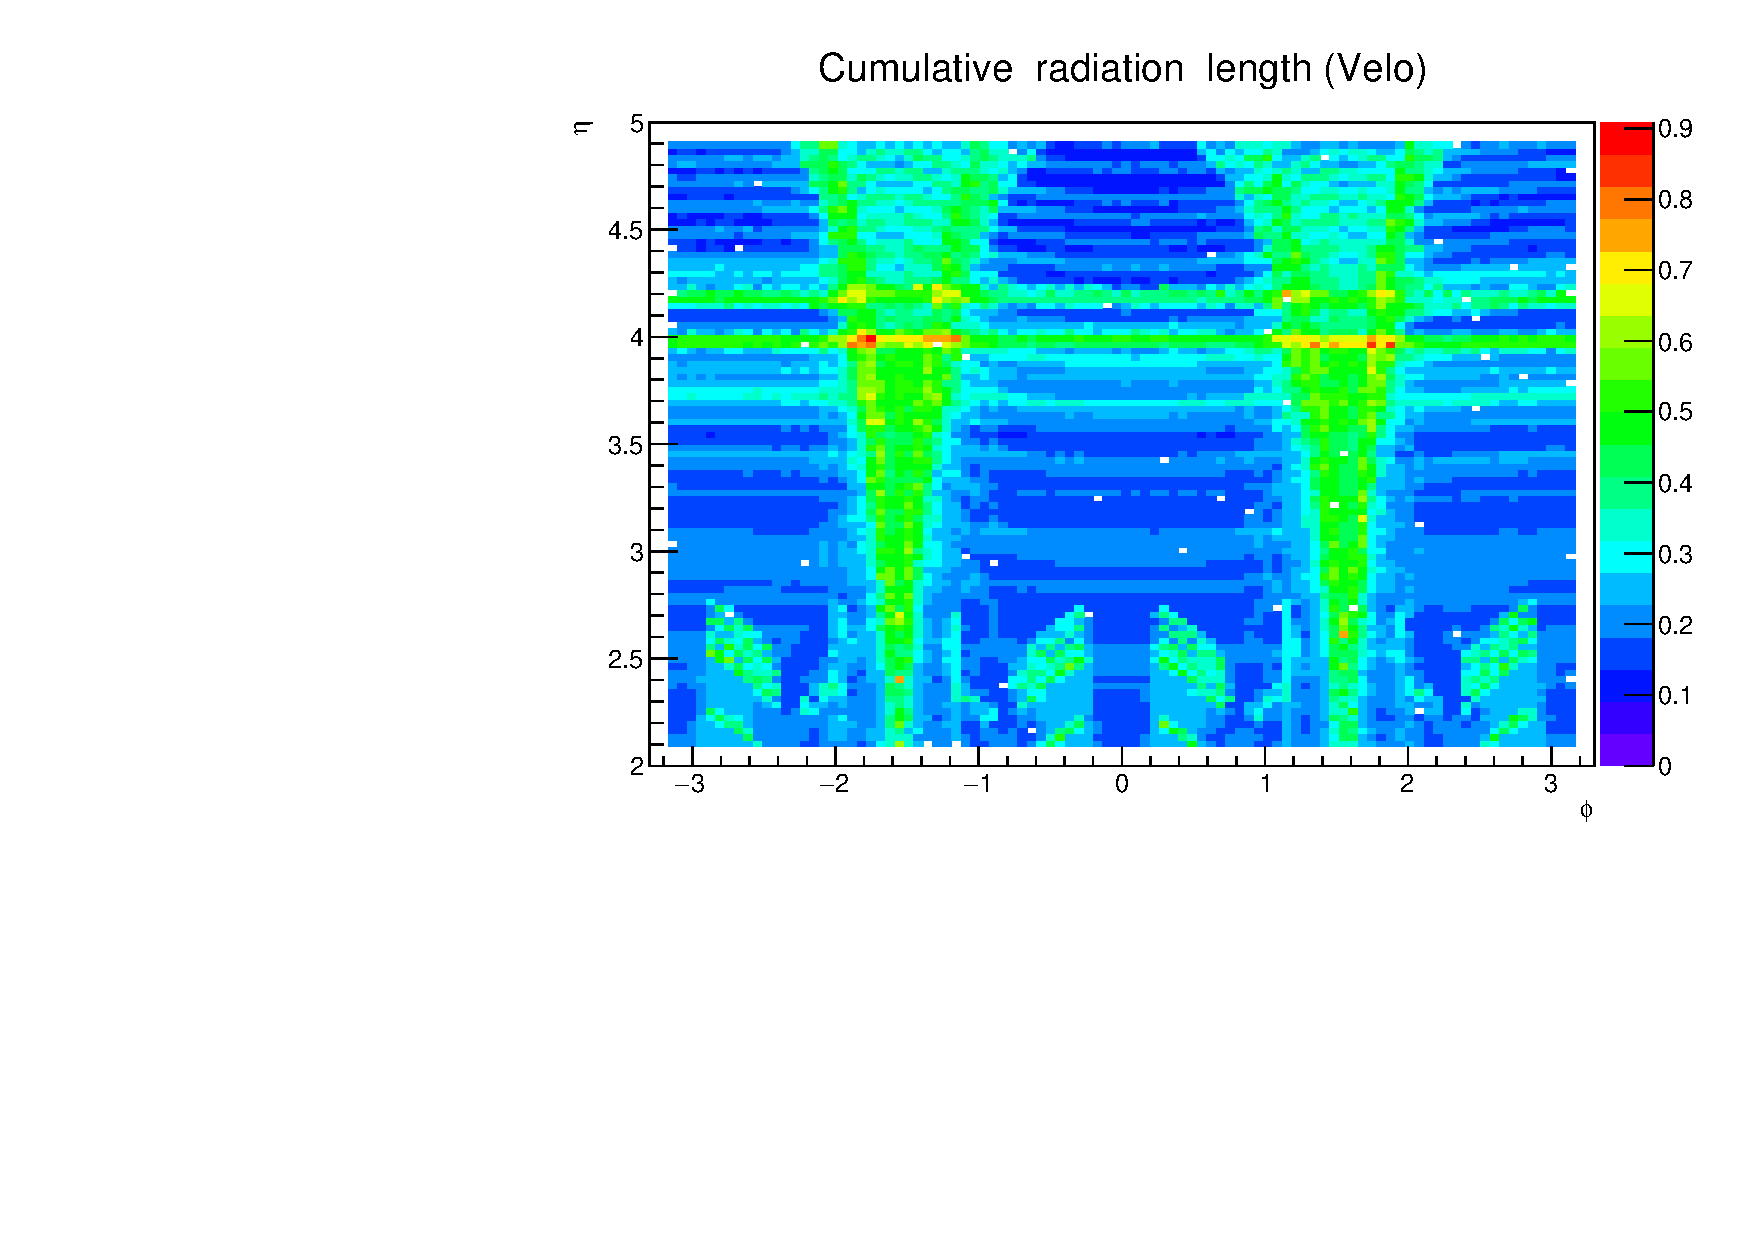
\includegraphics[width=0.8\textwidth]{Detector/figs/validation/radlenght/radlgh_prof_ID1.pdf}
\caption{Map of cumulative radiation length seen by a particle starting from
the interaction point up to the end of the VeLo.}
\label{fig:radlmap}
\end{figure}
%
Neutrinos are used as they do not bend in magnetic field and do not interact with the detector to any appreciable extent.
Thin air planes are inserted after each sub-detector. When these are traversed by the neutrinos, the information
about the accumulated radiation and interaction length is saved. In this way it is possible to obtain maps of
the detector, such as the one shown in Fig.~\ref{fig:radlmap}. Using the tool developed for this study
it is also possible to obtain the cumulative interaction length. 
% as a function of the position along the beam axis and the pseudorapidity. 
As an example Fig.~\ref{fig:cumradlZ} shows the average
radiation length as a function of the distance from the interaction point. Furthermore, it is possible to displace 
the primary vertex from its position, normally set at the origin, in order to study how this translates 
into the amount of material traversed. 

\begin{figure}[t]
\centering 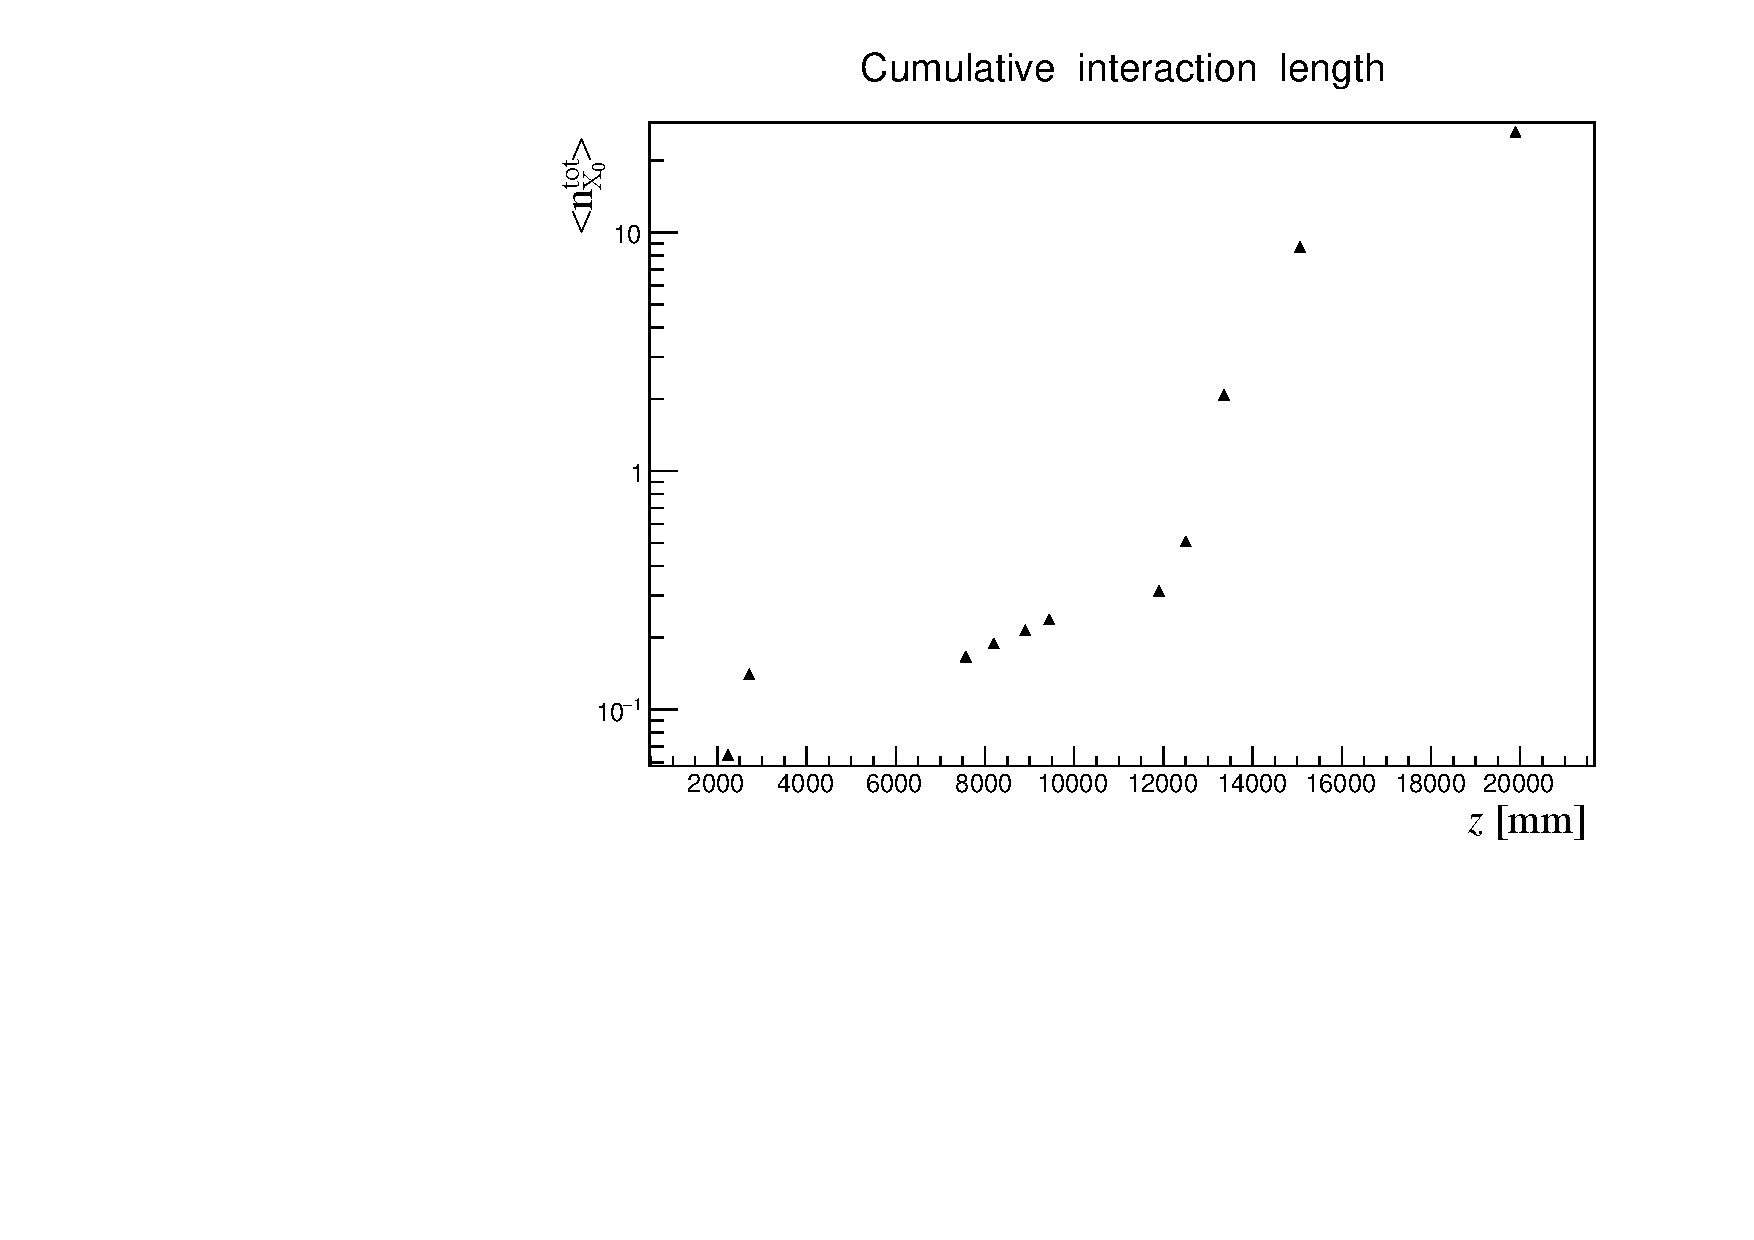
\includegraphics[width=0.8\textwidth]{Detector/figs/validation/radlenght/cuminterLength_vs_Z.pdf}
\caption{Average cumulative radiation length as a function of the horizontal 
distance from the interaction point. Each considered point corresponds to the end of a sub-detector:
VeLo, RICH1, RICH2, tracking stations, ECAL and HCAL and muon detector. }
\label{fig:cumradlZ}
\end{figure}


\section{Validation and material budget studies conclusions}
\label{sec:radlength_conlsusions}
The studies outlined in the previous two sections are based on tools which are now 
part of the standard LHCb simulation framework. These tools were used to validate 
the framework when passing from \textsc{Geant4} version 9.5 to version 9.6.
In particular a patch was provided by the \textsc{Geant4} team including
improved kaon cross-sections and it was verified these improve the agreement with data.
The tool will continue to be used in the future,
in particular to validate the upgrade to \textsc{Geant4} 10, in 2016.
Furthermore, the tools can be used by analyses sensitive to the quality of the simulation 
of particle and antiparticles cross-sections in order to study systematic effects and uncertainties.



